\documentclass[twoside]{article}

\usepackage{ustj}
\providecommand{\tightlist}{%
\setlength{\itemsep}{0pt}\setlength{\parskip}{0pt}}
\usepackage{fancyvrb}

\usepackage{tikz}
\newcommand{\bit}[1]{%
  \tikz[baseline=(char.base)]{%
    \node[shape=rectangle, draw, rounded corners=1pt, inner sep=1pt, minimum width=6pt, minimum height=6pt] (char) {#1};
  }%
}
\usepackage{subcaption}
\usepackage[edges]{forest}
\forestset{
    direction switch/.style={
        forked edges,
        for tree={
            calign=last,
            edge+=thick, 
            font=\sffamily,
        },
        where level=1{minimum width=13em}{},
        where level<=2{draw=red}{},
        where level>=1{folder, grow'=0}{},
    },
}
\usetikzlibrary{patterns}

\addbibresource{mss.bib}

\newcommand{\authorname}{Ted Blackman \patp{rovnys-ricfer},* \\ Joe Bryan \patp{master-morzod},† \\ Luke Champine \patp{watter-parter},* \\ Pyry Kovanen \patp{dinleb-rambep},† \\ Jose Cisneros \patp{norsyr-torryn},† \\ Liam Fitzgerald \patp{hastuc-dibtux}‡}
% \newcommand{\authorpatp}{\patp{sampel-palnet}}
\newcommand{\affiliation}{* Martian Engineering, \\ † Tlon Corporation, \\ ‡ Axiomatic Systems}

%  Make first page footer:
\fancypagestyle{firststyle}{%
\fancyhf{}% Clear header/footer
\fancyhead{}
\fancyfoot[L]{{\footnotesize
              %% We toggle between these:
              % Manuscript submitted for review.\\
              {\it Urbit Systems Technical Journal} III:1 (2026):  1–41. \\
              ~ \\
              Address author correspondence to \patp{rovnys-ricfer}.
              }}
}
%  Arrange subsequent pages:
\fancyhf{}
\fancyhead[LE]{{\urbitfont Urbit Systems Technical Journal}}
\fancyhead[RO]{Directed Messaging}
\fancyfoot[LE,RO]{\thepage}

%%MANUSCRIPT
\title{Directed Messaging}
\author{\authorname \\ \affiliation}
\date{}

\begin{document}

\maketitle
\thispagestyle{firststyle}

\begin{abstract}
\sloppy
Urbit's networking protocol was redesigned \mbox{achieving} over 100$\times$ throughput improvements while implementing content-centric networking in a production peer-to-peer system. Unlike address-based routing, all network operations (queries and commands) are expressed as remote namespace reads. Urbit's immutable scry namespace enables efficient caching, deterministic encryption, and stateless publishing, while a pre-distributed \textsc{pki} eliminates handshake overhead for single-roundtrip transactions. Lockstep Streaming, a novel scale-invariant packet authentication scheme using binary numeral trees, maintains authentication integrity across variable \textsc{mtu} sizes at relay hops. The Lackman traversal pattern enables constant-space streaming authentication. \mbox{Directed} routing simplifies peer discovery and \textsc{nat} traversal compared to previous approaches, while source-independent routing minimizes relay state. Begun in 2023 under the auspices of the Urbit Foundation and \mbox{deployed} in early 2025, Directed Messaging represents the first large-scale deployment of content-centric networking.
\end{abstract}

% We will adjust page numbering in final editing.
\pagenumbering{arabic}
\setcounter{page}{1}

\tableofcontents

\section{Introduction}

The Directed Messaging project was a fundamental overhaul of Urbit's networking stack. It rewrote the protocol definition and the protocol implementation, split between Hoon code inside Arvo (the Urbit overlay OS), and C code in Vere (the Urbit runtime).\footnote{The original Ames protocol is described in early detail in the Urbit whitepaper \citep{Whitepaper} with further elaboration in \patp{rovnys-ricfer}, ``Eight Years After the Whitepaper'', \ssc{ustj} vol. 1 iss. 1, pp.~1–46.} Directed Messaging addressed several major limitations of Urbit's previous networking stack: it increased throughput by over 100$\times$, improved peer discovery reliability, enabled the scalability of content delivery, and introduced a modular internal architecture that reduced implementation complexity. Directed Messaging is an encrypted, authenticated, peer-to-peer, packet-switched, message-oriented, connectionless, content-centric, transactional network protocol with its own congestion control, transmission control, and packet-level authentication. It was deployed to the Urbit network in early 2025.

\sloppy
These improvements were driven by Directed Messaging's total adherence to a request-response discipline throughout the stack, bundled with heavy use of Urbit's immutable referentially-transparent global namespace, called the ``scry namespace''. Every network message is either a request for data at a ``scry path'' (Urbit's equivalent of a \textsc{url}), or an authenticated response that includes the data at that path. This is true at the message layer and the packet layer, and for both reads (queries) and writes (commands).

Before Directed Messaging, the bandwidth Urbit was able to utilize was extremely limited, maxing out in the hundreds of kilobytes per second. It lacked orders of magnitude of performance in order to make effective use of commodity networking hardware, such as on a laptop or cloud instance. With Directed Messaging, Urbit's networking speed was able to reach over 1~Gibit/s on commodity hardware, sufficient for the vast majority of contemporary personal use cases.

Directed Messaging managed to improve throughput while preserving Urbit's already-good latency performance. For small messages, a network transaction is accomplished in one roundtrip: a command sent one way, followed by an acknowledgment the other way. Due to Urbit's public key infrastructure (\textsc{pki}) being disseminated to all nodes \emph{a priori} from a Byzantine fault-tolerant source (the Ethereum blockchain and a bespoke L2 for economic efficiency), no cryptographic handshake is needed for two Urbit nodes (called ``ships'' in Urbit lingo) to begin communication -- even their first exchange is a single roundtrip.

In addition to performance improvements, Directed Messaging scales better by leveraging runtime caching to disseminate data to many clients simultaneously. This strategy is particularly effective within Urbit's immutable scry namespace. Directed Messaging also introduces a new procedure for peer discovery and routing that is much more reliable and performant than the previous setups. It deals better with \textsc{nat} traversal and with using supernodes as relays more efficiently and reliably.

All of this is done by simplifying the basic networking structure to enforce a rigid request-response discipline throughout the entire system. In addition to that, it also places all network messages, including acknowledgments and commands, in addition to responses for queries asking for data, into the referentially transparent scry namespace. This makes Urbit's entire networking stack a named data networking system, which is also called content-centric networking. As far as the authors know, Directed Messaging is the very first production deployment of a content-centric networking protocol, as well as the deployment with the largest number of nodes. Not only that, its content-centricity preserves the immutability of Urbit's namespace throughout the stack. The immutability is key to the scalability improvements and reliability improvements, and it also helps with single-threaded performance.

\sloppy
Along the way, we designed and implemented a novel scheme for streaming packet authentication. This helps prevent denial-of-service attacks that could forge individual packets and spoof them in order to invalidate a large download. This attack is prevented by authenticating every packet, but unlike the previous version of Urbit's networking stack, which authenticated each packet with a signature (meaning one signature for every kilobyte of data, which was extremely inefficient), there's only one signature per message. A Merkelization scheme using binary numeral trees is used to authenticate the packets within that message \citep{Champine2021}.

This achieves a property that, to our knowledge, has not been demonstrated in prior packet authentication schemes: the ability to handle a different maximum transmission unit (\textsc{mtu}) at each hop in a relay chain without losing packet-level authentication. It is a scale-invariant packet-authentication scheme, and it also has good memory use characteristics, due to a novel algorithm based on the ``Lackman'' scale-invariant tree-traversal pattern developed by the authors. A relay receiving packets of one size and emitting packets of another size only needs to hold one large packet in memory while streaming (e.\,g.\ if receiving 1~kiB packets and sending 16kiB packets, it only needs to store 16~kiB of packet data at a time). It can seamlessly handle any \textsc{mtu} that is one kilobyte, two kilobytes, or any power-of-two number of kilobytes above that, up to 128~MiB.

Another advantage of the Directed Messaging protocol is that much more of the logic can be offloaded from the Urbit operating system, Arvo, into the runtime. This enables decoupling between the formal
specification, which is written in Nock, and implementation, which is written in C. This is in keeping with the spirit of Urbit's ``jet'' system that separates mechanism and policy for code execution. The most straightforward advantage of this decoupling is that each packet can be processed ephemerally, without incurring a disk write as in previous versions of Urbit's network protocol -- that was a severe bottleneck on the maximum throughput. The implementation in the runtime could be swapped out with another implementation written in another language, the congestion control algorithm could be swapped out, and parallelism strategies could readily be employed to increase multicore \textsc{cpu} utilization. The implementation that was deployed contains a major optimization: specialized arena allocators to reduce memory management overhead.

\section{High-Level Protocol Design}
\label{high-level-protocol-design}

\subsection{Request/Response, Namespace Reads}

The protocol design is based off the idea of a remote namespace read, wherein a ``subscriber'' ship requests data from a ``publisher'' ship, and the publisher sends that data as the response. The publisher ship makes the data available over the network by assigning it a path in Urbit's scry namespace and setting permissions appropriately (permissioning will be described fully in a later section). The subscriber ship, then, can download data from another ship by sending it a request for the data at a path and waiting for the response.

\sloppy
A network roundtrip is conceived of as a request, followed by a response. The request consists of a ``scry request'', i.\,e.\ a request for data at a scry path. An example scry path is  \lstinline[style=inlinecode]{/~zod/1/2/c/x/~2025.9.22/sys/kelvin}. A scry path immutably names a datum, in this case the \texttt{sys.kelvin} file published by \patp{zod} (at \texttt{rift=1} and \texttt{life=2}), within the \texttt{\%c} kernel module (Clay, the revision control system), with request type \texttt{\%x} (request file contents), and with timestamp at the start of the day on September 22, 2025. When a ship receives a scry request over the network, it can respond by sending a ``scry response'' containing the datum bound to that path.

Over the network, a network request is a single \textsc{udp} packet that encodes a scry path, limited to 384 characters so the request packet always fits into the internet-standard 1500-byte \textsc{mtu} (maximum transmission unit). A scry response may consist of a single packet, or multiple packets, depending on the size of the datum bound to that path. If the datum is 1kiB or less, the response is encoded into a single \textsc{udp} packet. Otherwise, the first scry response packet contains only the first 1kiB of the datum, along with a fixed-width field containing the number of bits in the whole datum.

If the subscriber ship receives a response indicating the datum is multi-packet, it switches modes and begins requesting the remainder of the datum, one~kiB at a time. Each request for a~kiB of data is itself a fully-fledged namespace read request, where the path in the request contains the path of the whole datum as well as the chunk size being requested (configured to 1~kiB over the public internet, but this could be increased to any power of 2~kiB's up to 128~MiB, for other environments, such as intra-datacenter). The protocol definition does not require those fragment requests to be sent in any particular order or according to any particular congestion control algorithm. The current implementation uses a packet-switched variant of the \textsc{tcp} NewReno congestion control algorithm, written in C in Urbit's runtime, to manage multi-packet reads. The message-level authentication is sent in the first response packet. Each subsequent packet is authenticated as being part of that message by using the LockStep streaming authentication scheme, described in a later section.

This remote read flow is a ``pure read'': handling a read request does not require the publisher ship to change any persistent state. But a general-purpose network protocol needs to be able to express commands, not just reads. Directed Messaging builds commands out of reads. A command is conceived of as two reads, one in each direction:

\begin{enumerate}
  \item  The ship sending the command makes the command datum available within its own scry namespace, so the receiving ship has the ability to read the command by sending a remote read request.
  \item  The ship that receives the command, after attempting to execute the command, makes the command's result available within its namespace, so the sending ship has the ability to read the result (hereafter called the ``ack'') by sending a remote read request. A result can be success (``ack'') or an error datum (``naxplanation'', named after ``nack'' for negative acknowledgment).
\end{enumerate}

This approach is conceptually clean but immediately presents two practical challenges. The first is triggering: how does the receiving ship \emph{know} to request the command datum from the sending ship? There are many ships on the network; it would be absurdly impractical to send requests to all of them on the off-chance that one or two of them have an outstanding command for us. The second challenge is latency: a naive implementation would imply every command requires two network roundtrips, one to remote-read the command and one to remote-read the command's result (ack or naxplanation). If so, that would be unfortunate, since Urbit's previous networking required only one roundtrip for a command and ack, in the common case of a small (≤1~kiB) command datum, and unneeded roundtrips are anathema to
a good user experience \citep{Cheshire1996}.

Fortunately, we can solve both problems with one weird trick. We add a ``request type'' bit to each network request packet indicating whether it is a read or a command, and if it is a command, it includes not only the scry request path, but also a scry response containing the first 1~kiB of the command datum. When the receiving ship's runtime receives the packet, it looks at the `request-type' bit to determine how to handle the packet.

If the incoming request packet is a read, the runtime performs a read request on the Arvo OS by firing its \lstinline[style=inlinecode]{+peek} arm, a Nock function that reads from Arvo's namespace. This read request does not trigger any disk writes and could be run in parallel with other reads and with an Arvo event. The runtime then encodes the result of this read as a scry response packet and sends it back to the IP and port that sent the request.

If the packet is a command, the runtime injects the packet as a stateful Arvo ``event'' by firing its \lstinline[style=inlinecode]{+poke} arm (a Nock function that sends an event or command for Arvo to process, producing effects and a new Arvo OS with a modified state). When this event completes, one of the effects it produces can be a scry response packet containing the ack, which the runtime will send back to the IP and port that sent the request.

If the command datum fits within 1~kiB, the entire command is sent in the first packet, recapturing the single-roundtrip flow for a command and an ack. Multi-packet commands are downloaded by the commanded ship using the same congestion control as downloading any other potentially large datum -- and, importantly, those incremental downloads do not necessarily trigger unnecessarily frequent disk writes.

\section{Routing}
\label{routing}

\subsection{Directed Routing}
\label{directed-routing}

The Directed Messaging protocol gets its name from its routing scheme, which treats each bidirectional communication between two Urbit ships as directed, like a directed edge in a graph. For each request/response roundtrip, one ship is the requester, and the other is the responder, and that distinction is known at every layer of the system. Making this directionality known to routing enables a routing paradigm where a response packet traces the exact same relay path through the network as the request path, in the reverse order. Previous Urbit networking protocols used the opposite paradigm: ``criss-cross routing'', so-called because both request and response could be routed through the destination ship's ``sponsor'', i.\,e.\ the supernode ship (``galaxy'' root node or ``star'' infrastructure node) responsible for relaying packets to that ship. In contrast, in directed routing, the request and the response both use the same relay: the responder ship's sponsor.  See Figure~\ref{fig:routing-strategies} for a comparison of the two routing strategies.

\begin{figure}
  \centering
  \vspace{1cm}
  \begin{subfigure}{\textwidth}
    \centering
    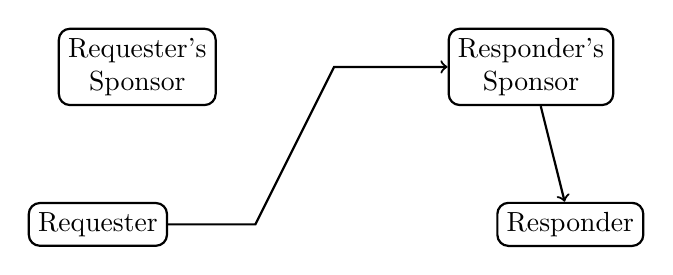
\begin{tikzpicture}[align=center]
      % draw a rounded rectangle around the label
      \node[draw, thick, rounded corners] (R) at (-3,-1) {Requester};
      \node[draw, thick, rounded corners] (RS) at (-2.5, 1) {Requester's\\ Sponsor};
      \node[draw, thick, rounded corners] (Res) at (3,-1) {Responder};
      \node[draw, thick, rounded corners] (ResS) at (2.5, 1) {Responder's\\ Sponsor};
      
      \coordinate (R1) at (-1,-1);
      \coordinate (R2) at (0,1);   

      \draw[->, thick, inner sep=0, outer sep=0] (R) -- (R1) -- (R2) -- (ResS);
      \draw[->, thick, inner sep=0, outer sep=0] (ResS) -- (Res);
    \end{tikzpicture}
    \subcaption{Request (same for both directed and criss-cross routing).  \vspace{1cm}}
  \end{subfigure}
  \begin{subfigure}{\textwidth}
    \centering
    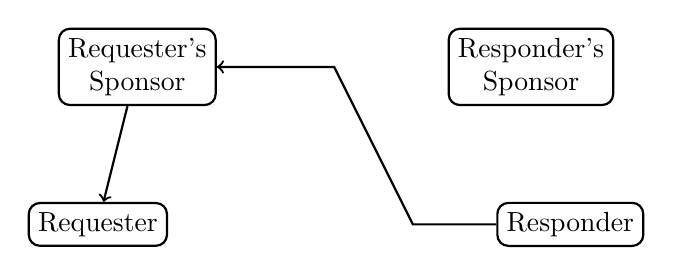
\begin{tikzpicture}[align=center]
      \node[draw, thick, rounded corners] (R) at (-3,-1) {Requester};
      \node[draw, thick, rounded corners] (RS) at (-2.5, 1) {Requester's\\ Sponsor};
      \node[draw, thick, rounded corners] (Res) at (3,-1) {Responder};
      \node[draw, thick, rounded corners] (ResS) at (2.5, 1) {Responder's\\ Sponsor};

      \coordinate (Res1) at (1,-1);
      \coordinate (Res2) at (0,1);   

      \draw[->, thick, inner sep=0, outer sep=0] (Res) -- (Res1) -- (Res2) -- (RS);
      \draw[->, thick, inner sep=0, outer sep=0] (RS) -- (R);
    \end{tikzpicture}
    \caption{Response (criss-cross routing).  \vspace{1cm}}
  \end{subfigure}
  \begin{subfigure}{\textwidth}
    \centering
    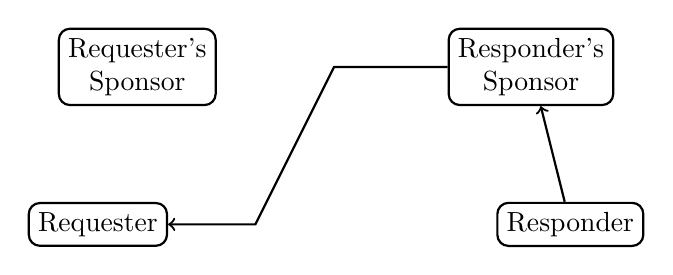
\begin{tikzpicture}[align=center]
      \node[draw, thick, rounded corners] (R) at (-3,-1) {Requester};
      \node[draw, thick, rounded corners] (RS) at (-2.5, 1) {Requester's\\ Sponsor};
      \node[draw, thick, rounded corners] (Res) at (3,-1) {Responder};
      \node[draw, thick, rounded corners] (ResS) at (2.5, 1) {Responder's\\ Sponsor};

      \coordinate (R1) at (-1,-1);
      \coordinate (R2) at (0,1);   

      \draw[->, thick, inner sep=0, outer sep=0] (ResS) -- (R2) -- (R1) -- (R);
      \draw[->, thick, inner sep=0, outer sep=0] (Res) -- (ResS);
    \end{tikzpicture}
    \caption{Response (directed routing).}
  \end{subfigure}
  \caption{Routing strategies.}
  \label{fig:routing-strategies}
\end{figure}

% \subsubsection{Request (Same for both Directed and Criss-Cross
% Routing)}\label{request-same-for-both-directed-and-criss-cross-routing}

% \begin{lstlisting}[style=listingblock]
% requester's sponsor       -------- responder's sponsor
%                          /             \
% requester  ------------                 ---> responder
% \end{lstlisting}

% \subsubsection{Response (Directed Routing)}\label{response-directed-routing}

% \begin{lstlisting}[style=listingblock]
% requester's sponsor       -------- responder's sponsor
%                          /             \
% requester  <-----------                 ---- responder
% \end{lstlisting}

% \subsubsection{Response (Criss-Cross
% Routing)}\label{response-criss-cross-routing}

% \begin{lstlisting}[style=listingblock]
% requester's sponsor -----          responder's sponsor
%                 /          \
% requester <---              ---------------  responder
% \end{lstlisting}

\subsection{Relaying}\label{relaying}

Making the directedness of communication legible to relays and Urbit runtimes allows the protocol to be a faithful, if Urbit-specific, Named Data Networking (\textsc{ndn}) protocol, which had been Urbit's stated goal since 2010. A Directed Messaging request packet acts as an \textsc{ndn} ``interest'' packet, and a response packet acts as an \textsc{ndn} ``data'' packet.

The \textsc{ndn} family of protocols, created by Van Jacobson~et~al. in the mid-2000s, differs from traditional networking protocols in that an interest packet has no sender address field -- the identity of the sender of a request is unknown to the network. Instead, a receiver (relay or server) remembers ``where'' it heard the request from, and sends the response back to that. The notion of ``where'' varies depending on the layer of the stack the system is operating at: for an IP replacement, a relay would remember the physical interface (e.\,g.\ Ethernet port) on which it heard the incoming request. When building on top of IP and \textsc{udp}, as Directed Messaging does, a receiver remembers the IP and port of the sender.

Previous Urbit network protocols still included the sender's Urbit identity in the request packets, failing to achieve the ``source independence'' property that defines \textsc{ndn}. Directed Messaging is completely source-independent for reads, and for commands, it piggybacks a source-independent response onto a source-independent request in such a way that the receiver does know which Urbit address sent the request, but not in a way that requires packet routing to know or use the source Urbit address.

Source independence lets the routing operate fully locally, without reference to or knowledge of anything beyond a single hop away in either direction. This minimizes the data storage and synchronization requirements for nodes, which could become significant at scale.

Source independence entails stateful routing. Directed Messaging adopts \textsc{ndn}'s Pending Interest Table, which stores a mapping from each outstanding request to the IP and port that sent that request. If the request times out (after roughly 30 seconds), or the request is satisfied by a response, the request is deleted from the table.

Since responses are authenticated down to the packet level, and immutable (meaning no cache invalidation is ever needed, only eviction), it should be straightforward for relays to cache responses, enabling efficient content distribution through the network. At present, each Urbit ship's runtime has a cache for its own responses, but supernodes (galaxies and stars) do not yet cache responses from their sponsored ships.

\subsection{Peer Discovery}\label{peer-discovery}

Urbit is a peer-to-peer network. Only root nodes (galaxies) list their own IP addresses publicly (on the Ethereum blockchain); all other ships must be discovered on demand. When one ship first sends a request to another ship, it generally doesn't know at what IP and port that ship could be reached, and it also doesn't know if the ship is reachable directly, or behind a firewall and only reachable through its sponsor.

The criss-cross routing used in previous Urbit protocols was hard to work with in practice and suffered from inefficiencies and bugs. Directed Messaging has a simpler approach to peer discovery that is easier to reason about.

The main difficulties with criss-cross routing stem from the  structure of the internet. Most residential internet connections live behind a firewall that blocks all unsolicited incoming \textsc{udp} packets. A laptop at home can send an outgoing packet to some destination IP and port, and the router will relay response packets back to the laptop for some time afterward, usually 30 seconds, as long as those response packets come from that same destination IP and port.

A \textsc{udp}-based peer-to-peer network, then, needs to include not only residential nodes but also nodes on the public internet, not behind firewalls. These nodes must be discoverable so that residential nodes can ping them every 25 seconds, to ensure the residential nodes can receive messages. In Urbit, these public nodes are the galaxies (root nodes) and stars (infrastructure nodes). For now, only galaxies perform routing, due to edge cases with two levels of supernodes in peer discovery using criss-cross routing -- we expect Directed Messaging will unblock stars from participating in routing.

When communicating with another ship for the first time, a ship first sends the packet to the other ship's sponsoring galaxy, which has an open connection to its sponsored ship if it's online. The galaxy receives a ping every 25 seconds from its sponsored ship. Whenever the source IP and port change, the galaxy's runtime injects an Arvo event and its Arvo OS saves the sponsored ship's new location to disk.

In Directed Messaging, when the galaxy receives a packet intended for one of its sponsored ships, it relays the packet. This uses the pending interest table described above to track the fact that there is an outstanding request that the galaxy is expecting to be honored by a response from the sponsored ship. The fundamental invariant of directed routing is that the response packet must trace the exact same path through the network as the request packet had, just reversed. Since this request had gone through this galaxy, the response must also route through the galaxy.

\sloppy
In Urbit's previous protocols, in contrast, the response would go directly from the sponsored ship back to the requesting ship, and also potentially through the requesting ship's sponsoring galaxy. This works in principle, but one drawback has to do with ``route tightening'' (described below): the response route only tightens to a direct route (without relays) if there are requests flowing in both directions; otherwise every response will flow through the requester's sponsor, even if the requester is not behind a firewall.

\subsection{Route Tightening}
\label{route-tightening}

It is better for performance, scaling, and individual sovereignty to
obtain a direct route to another ship, rather than communicating through
relays. In order to facilitate this, the system must automatically
``tighten'' a route over time to reduce the number of hops. Directed
Messaging accomplishes this in the relay. When a relay receives a
response packet (originally sent by a transivitely sponsored ship, but
possibly through a relay once stars begin relaying packets), it appends
the IP and port from which it heard that packet to the end of the packet
before forwarding it to the requesting ship. Once the requesting ship
receives this augmented packet, it knows the address appended to that
packet is next hop in the relay chain. Once it knows that, when it sends
packets to the responding ship, it can send them through the first hop
in the relay chain (the receiving ship's galaxy), or to the next hop,
which could be another relay or the ship itself.

In the current implementation, the requesting ship uses a simple
procedure to decide which routes to send the packet on. It tracks the
date of the last received packet from both the direct route and the
route through the galaxy. A route is considered active if a packet has
been received on it within the last five seconds. When the requesting
ship goes to send a packet, if the direct route is active, it sends the
packet on that route. Otherwise, it sends the packet through the galaxy
and also sends a copy of the packet on the direct route as a probe.

This ensures continuity of communication when switching to or from a
direct route, and it automatically tightens to the direct route if the
direct route is responsive and loosens to the galaxy route if the direct
route becomes unresponsive.

\section{Authentication and
Encryption}\label{authentication-and-encryption}

Directed Messaging is always authenticated and supports encryption in a number of different modes:
\begin{itemize}
  \item  \textbf{Unencrypted reads}: A ship can publish data into its namespace without encryption. Response messages are signed using the ship's private key. The signature attests to the scry binding: the pair of the scry path and the datum at that path.
  \item  \textbf{One-to-One Encrypted Reads}: A ship can make data available to a single peer ship. Response messages are authenticated via an external hash-based message authentication code (\textsc{hmac}) and internal signature. They are encrypted using a symmetric key derived from the Diffie-Hellman key exchange of the two ships' keys.
  \item \textbf{Commands}: Commands and their acks are both handled as one-to-one encrypted reads.
  \item \textbf{One-to-Many Encryption}: A ship can make data available to many ships by sharing an encryption key for that data to each ship using a one-to-one encrypted read. The requesting ship then uses that key to encrypt the request's scry path and decrypt the scry response.
\end{itemize}

The core encryption primitives consist of:

\begin{itemize}
  \item  \texttt{kdf}: BLAKE3, in its key derivation mode.
  \item  \texttt{crypt}: XChaCha8, with its 24-byte nonce derived by processing the (arbitrary-length) input initialization vector (IV) using the key derivation function (\texttt{kdf}) with \texttt{"mesa-crypt-iv"} as the context string.
\end{itemize}

\noindent
Messages and their paths are encrypted separately. First, \texttt{kdf} is used to derive an authentication key and encryption key from the shared secret. The authentication key is used to compute a 128-bit keyed BLAKE3 hash of the path; this serves as the Authenticated Encryption with Associated Data (\textsc{aead}) tag. The encryption key is then used to encrypt the path with \texttt{crypt}, using the tag as the IV. Concatenating the encrypted path and authentication tag yields a ``sealed'' path. The message itself is then encrypted with \texttt{crypt}, using the sealed path as the IV. Authentication of the message is achieved via a Merkle hashing scheme described later.

Directed Messaging's encryption scheme uses a variant of ChaCha20, XChaCha, with reduced rounds for performance. XChaCha is an extended-nonce variant of ChaCha that accepts a 192-bit nonce instead of the standard 96-bit nonce. However, rather than using the caller-provided initialization vector directly as the nonce, Directed Messaging first applies a BLAKE3 key derivation function to derive a deterministic 24-byte nonce from the IV using the context string \texttt{"mesa-crypt-iv"}. This XChaCha operation with 8 rounds then produces a derived key and extended nonce, which are subsequently used for the actual ChaCha encryption (also with 8 rounds) of the message payload. The use of 8 rounds instead of the standard 20 is a performance optimization -- ChaCha's security margin allows for this reduction in cryptographic applications where the extreme paranoia of 20 rounds may be unnecessary \citep{Aumasson2019}, and the deterministic nonce derivation via BLAKE3 adds an additional layer of domain separation.

Because the scry namespace immutably binds paths to their message data, the path serves as a synthetic IV for the message, making encryption deterministic. This solves multiple problems.  It (along with other principles of Directed Messaging) prevents replay attacks by construction. Every Directed Messaging packet is idempotent at the application level (a duplicate packet can trigger a duplicate ack and minor state changes in the runtime and Arvo kernel related to routing state, but it cannot modify anything visible to an application). It further removes the need for explicit nonce management, such as generating, storing, and transmitting an explicit nonce for each message. Not tracking nonces reduces the system's security attack surface area considerably, since nonce state mismanagement is a common source of vulnerabilities. Finally, supporting encrypted values in the namespace allows the system to implement encryption using overlay namespaces (described in more detail below), which provide a clean layering that separates encryption from other concerns.

Before transmission, a single \texttt{0x1} byte is appended to the encrypted message, called a ``trailer byte''. This solves a representation problem specific to Urbit's atom system. In Urbit, data is ultimately stored as ``atoms'': arbitrary-precision natural numbers. The atom system cannot distinguish between byte streams with equivalent numerical value; that is, it has no way to ``say'' \texttt{0x1000} instead of \texttt{0x1} or \texttt{0x1000000000} -- all are numerically equivalent to 1.\footnote{Note the relative most-significant byte (\textsc{msb}) order notation used here, contrary to Urbit's customary \textsc{lsb} order.} Thus, if a ciphertext happens to end with one or more zero bytes, those would be stripped when the ciphertext is represented as an atom, corrupting the data. Appending a 0x1 byte ensures that the atom representation always preserves the full length of the ciphertext, including any trailing zeros. During decryption, the code verifies that the final byte is indeed \texttt{0x1} (which catches truncation or corruption) and then strips it before decrypting.  This construction provides authenticated encryption properties through the deterministic relationship between the IV and nonce, ensuring that any tampering with the ciphertext or IV will result in decryption failure.

\subsection{Message Authentication and Encryption
Details}\label{message-authentication-and-encryption-details}

\subsubsection{Overlay Namespaces}\label{overlay-namespaces}

Each of the three privacy modes has its own ``overlay namespace'', i.\,e.\ a part of the scry namespace that somehow transforms values bound to a different part of the namespace. A path in an overlay namespace often consists of a path prefix containing the name of the overlay and any parameters needed for the transformation it performs on the datum at the overlaid path, followed by the overlaid path.

A handler function that deals with scry requests to the overlay namespace is free to parse transformation parameters out of the overlay prefix, inspect the overlaid path, make a scry request for the data at that path, make scry requests related to that path (such as existence checks for file paths), and run arbitrary code to transform the results. This is all possible because scry requests are purely functional by construction -- they are deterministic functions of their inputs, with no hidden inputs, and there is no mechanism by which they could change Arvo state.

Directed Messaging uses overlay namespaces not only for privacy modes, but also to publish individual packets within a message. The packet's size (expressed as the log base 2~kiB, e.\,g.\ 3 for 8~kiB or 4 for 16~kiB) and fragment number (index within the message) are parameters to this overlay, which overlays the message's scry path.

Directed Messaging is the first Urbit kernel module to make heavy use of overlay namespaces in its design. They play an important role in maintaining boundaries between layers within the system: privacy is separated, by construction, from other concerns due to the isolation imposed by overlay namespaces. For example, an application can declare what privacy mode it wants to use for a piece of data it publishes, and the kernel enforces that by exposing it over the network using the appropriate overlay namespace.

\subsubsection[\texttt{\%publ} namespace (unencrypted public)]{\texttt{\%publ} namespace (unencrypted public)}
\label{publ-namespace-unencrypted-public}

A value registered in the \lstinline[style=inlinecode]{%publ} namespace is intended to be publicly readable by anyone on the network.  The message is not encrypted, but it is authenticated using signature authentication only (using a 64-byte Ed25519 signature calculated over the encoded beam path and the \textsc{lss} root of the unencrypted jammed data).  The publisher signs the message using their Ed25519 private key (extracted from their networking key), and the receiver verifies the signature using the publisher's Ed25519 public key retrieved from Azimuth.  In this model, authenticity is provided by the signature, while confidentiality is not provided since the message is sent in plaintext.

The \texttt{\%publ} namespace uses unencrypted paths with the structure:

\begin{lstlisting}[style=listingblock]
/publ/[life]/[path]
\end{lstlisting}

\noindent
with the components:
\begin{itemize}
  \item  \lstinline[style=inlinecode]{life} (key revision number) of the publisher's networking keys is used to identify which public key to use for signature verification.
  \item  \lstinline[style=inlinecode]{path} is the actual user path in plaintext.  This is not encrypted and is visible to all network observers.
\end{itemize}

Everything in the \lstinline[style=inlinecode]{%publ} namespace is public:  both the publisher's identity/key version and the content path are visible to anyone. No encryption is applied to either the path or the message payload. Authentication comes solely from the Ed25519 signature, which proves the publisher created this content. Key rotation is supported through the life counter.

Its use cases include public data that should be readable by anyone, content where authenticity matters but confidentiality doesn't, and scenarios where simplicity is preferred over the complexity of encrypted namespaces (since no key exchange or group key distribution is required).

\subsubsection{\texttt{\%shut} namespace (group encrypted)}
\label{shut-namespace-group-encrypted}

In contrast, the \lstinline[style=inlinecode]{%shut} namespace is intended for one-to-many encrypted data sharing, wherein a publisher ship shares data with a group of ships by encrypting the data with a shared symmetric key known to the group.  The message is encrypted with XChaCha8 using this group symmetric key.  The key is provided via the \lstinline[style=inlinecode]{%keen} task (not derived from \textsc{ecdh}).  The encrypted path indicates which group key to use.  Signature authentication takes place using a 64-byte Ed25519 signature computed over the encoded beam path and the \textsc{lss} root of the encrypted data.  The signature uses the publisher's Ed25519 private key, proving that the publisher created this encrypted payload.  The receiver verifies the signature using the publisher's Ed25519 public key from Azimuth, then decrypts with the group key.  In this security model, the signature proves authenticity from the publisher, while encryption provides confidentiality to group members.  Anyone with the group key can decrypt, but only the publisher can create valid signatures.

The \lstinline[style=inlinecode]{%shut} namespace uses encrypted paths with the structure:

\begin{lstlisting}[style=listingblock]
/shut/[key-id]/[encrypted-path]
\end{lstlisting}

\noindent
with the components:
\begin{itemize}
  \item  \lstinline[style=inlinecode]{key-id}: A numeric identifier indicating which group symmetric key to use for decryption. This allows multiple groups to be supported, each with their own key.
  \item  \lstinline[style=inlinecode]{encrypted-path}: The actual user path, encrypted using the group key.  This is sealed with the same symmetric key used to encrypt the message payload, making the entire scry path opaque to anyone without the group key.
\end{itemize}

\noindent
The actual content path is hidden from network observers. Only the key ID is visible in plaintext.  The group key must be obtained separately (typically via a \lstinline[style=inlinecode]{%keen} task) to decrypt both the path and the message payload. Different groups using different key IDs can coexist without revealing which content is being accessed.

\subsubsection{\texttt{\%chum} namespace (1-to-1 encrypted)}
\label{chum-namespace-1-to-1-encrypted}

The \lstinline[style=inlinecode]{%chum} namespace is intended for one-to-one encrypted data sharing between two ships.  Authentication utilizes \textsc{hmac} only (without signatures).  The message is encrypted with XChaCha8 using a symmetric key derived from Curve25519 \textsc{ecdh} key exchange between the two ships' networking keys.  A 16-byte \textsc{hmac} (BLAKE3 keyed hash) is computed over the encoded beam path and the \textsc{lss} root of the encrypted data, using the same \textsc{ecdh}-derived symmetric key. Both parties can independently derive this key from their own private key and the other party's public key. The receiver verifies the \textsc{hmac} using the shared symmetric key, then decrypts with the same key.  In this security model, the \textsc{hmac} proves the sender possesses the shared symmetric key (implicitly authenticating them as the expected peer). No signatures are needed since only two parties share this key. This applies to both pokes and acks.

The \lstinline[style=inlinecode]{%chum} namespace uses encrypted paths with structure:

\begin{lstlisting}[style=listingblock]
/chum/[server-life]/[client-ship]/[client-life]/
  [encrypted-path]
\end{lstlisting}

\noindent
with the components:
\begin{itemize}
  \item  \lstinline[style=inlinecode]{server-life}: The life (key revision number) of the server ship's networking keys, used to identify which version of their keys to use for \textsc{ecdh} key derivation.
  \item  \lstinline[style=inlinecode]{client-ship}: The \texttt{@p} address of the client ship in the communication pair.
  \item  \lstinline[style=inlinecode]{client-life}: The life of the client ship's networking keys, used to identify which version of their keys to use for \textsc{ecdh} key derivation.
  \item  \lstinline[style=inlinecode]{encrypted-path}: The actual user path, encrypted using the symmetric \textsc{ecdh} key derived from both ships' networking keys. This makes the scry path opaque to network observers.
\end{itemize}

\noindent
This arrangement yields some nice privacy properties.  The actual content path is hidden from network observers. Only the identities of both parties and their key versions are visible in plaintext.  Only the two ships involved can derive the symmetric key to decrypt the path and payload. Key rotation is supported through the life counters.

\subsubsection{Other Cryptographic Properties}
\label{other-cryptographic-properties}

Directed Messaging relies on the ability to rotate keys on chain for its forward secrecy. Future versions of the protocol might add a ratchet to minimize the damage if a private key is compromised.

\subsection{Packet Authentication}
\label{packet-authentication}

One of the goals of Directed Messaging was to improve upon the
safe but dumb conservative design of old Ames to sign every 1~KiB packet. The standard approach is to use asymmetric crypto to establish a shared \textsc{aead} key, and use it to authenticate each packet. This is just as safe as signing every packet, and orders of magnitude faster. However, one still can't verify that a peer is sending \emph{correct} data until one has received the entire message. The remote could send 999 good packets and one bad, and the receiver has no way of knowing which was which. This is especially annoying if one wants to download in parallel from multiple peers: if the final result is invalid, which peer is to blame?

Verifying that a packet belongs to a particular message is a job for a Merkle tree. Thus the protocol needs to split message data into the leaves of a tree, and send both leaf data and tree hashes. Early on, we debated whether to make these distinct request types; we settled on interleaving them. Now the question becomes: which tree hashes does one need to send, and when does one send them?

The relevant design constraints were:
\begin{enumerate}
  \item  Sufficiently-small messages should not require more than one packet.
  \item  It should be possible to download in parallel.
  \item  The protocol should be flexible with respect to the size of a leaf.
\end{enumerate}

\noindent
An obvious first place to look for inspiration was \href{https://github.com/oconnor663/bao}{Bao} \citep{oconnor663}. However, Bao is not very amenable to being split into fixed-size packets: it intermingles leaf data and tree hashes into one stream, and the number of consecutive hashes varies based on the offset. You could modify it such that each packet consists of a leaf followed by at most one hash; indeed, this was the initial plan. Visually:

%                        ┌──────────────┴─────────────a
%            ┌───────────┴───────────b              ┌─┴─q
%      ┌─────┴─────c           ┌─────┴─────j        │   │
%   ┌──┴──d     ┌──┴──g     ┌──┴──k     ┌──┴──n     │   │
% ┌─┴─e ┌─┴─f ┌─┴─h ┌─┴─i ┌─┴─l ┌─┴─m ┌─┴─o ┌─┴─p ┌─┴─r │
% 0   1 2   3 4   5 6   7 8   9 10 11 12 13 14 15 16 17 18

\noindent
\hspace{3pt}
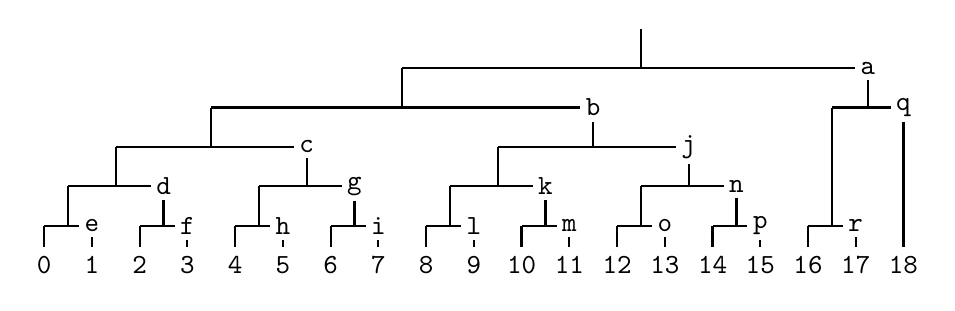
\begin{tikzpicture}[
  x=0.05\textwidth,
  y=1cm,
]
  \coordinate (root) at (12.5, 3.0) {};

  \coordinate(al) at (7.5, 2.5) {};
  \coordinate(ac) at (12.5, 2.5) {};
  \coordinate (ar) at (17.25, 2.5) {};

  \coordinate (bl) at (3.5, 2.0) {};
  \coordinate (bc) at (7.5, 2.0) {};
  \coordinate (br) at (11.5, 2.0) {};
  \coordinate (ql) at (16.5, 2.0) {};
  \coordinate (qc) at (17.25, 2.0) {};
  \coordinate (qr) at (18, 2.0) {};

  \coordinate (cl) at (1.5, 1.5) {};
  \coordinate (cc) at (3.5, 1.5) {};
  \coordinate (cr) at (5.5, 1.5) {};
  \coordinate (jl) at (9.5, 1.5) {};
  \coordinate (jc) at (11.5, 1.5) {};
  \coordinate (jr) at (13.5, 1.5) {};

  \coordinate (dl) at (0.5, 1.0) {};
  \coordinate (dc) at (1.5, 1.0) {};
  \coordinate (dr) at (2.5, 1.0) {};
  \coordinate (gl) at (4.5, 1.0) {};
  \coordinate (gc) at (5.5, 1.0) {};
  \coordinate (gr) at (6.5, 1.0) {};
  \coordinate (kl) at (8.5, 1.0) {};
  \coordinate (kc) at (9.5, 1.0) {};
  \coordinate (kr) at (10.5, 1.0) {};
  \coordinate (nl) at (12.5, 1.0) {};
  \coordinate (nc) at (13.5, 1.0) {};
  \coordinate (nr) at (14.5, 1.0) {};

  \coordinate (el) at (0, 0.5) {};
  \coordinate (ec) at (0.5, 0.5) {};
  \coordinate (er) at (1, 0.5) {};
  \coordinate (fl) at (2, 0.5) {};
  \coordinate (fc) at (2.5, 0.5) {};
  \coordinate (fr) at (3, 0.5) {};
  \coordinate (hl) at (4, 0.5) {};
  \coordinate (hc) at (4.5, 0.5) {};
  \coordinate (hr) at (5, 0.5) {};
  \coordinate (il) at (6, 0.5) {};
  \coordinate (ic) at (6.5, 0.5) {};
  \coordinate (ir) at (7, 0.5) {};
  \coordinate (ll) at (8, 0.5) {};
  \coordinate (lc) at (8.5, 0.5) {};
  \coordinate (lr) at (9, 0.5) {};
  \coordinate (ml) at (10, 0.5) {};
  \coordinate (mc) at (10.5, 0.5) {};
  \coordinate (mr) at (11, 0.5) {};
  \coordinate (ol) at (12, 0.5) {};
  \coordinate (oc) at (12.5, 0.5) {};
  \coordinate (or) at (13, 0.5) {};
  \coordinate (pl) at (14, 0.5) {};
  \coordinate (pc) at (14.5, 0.5) {};
  \coordinate (pr) at (15, 0.5) {};
  \coordinate (rl) at (16, 0.5) {};
  \coordinate (rc) at (16.5, 0.5) {};
  \coordinate (rr) at (17, 0.5) {};

  \node[draw=none] (n0) at (0,0) {\texttt{0}};
  \node[draw=none] (n1) at (1,0) {\texttt{1}};
  \node[draw=none] (n2) at (2,0) {\texttt{2}};
  \node[draw=none] (n3) at (3,0) {\texttt{3}};
  \node[draw=none] (n4) at (4,0) {\texttt{4}};
  \node[draw=none] (n5) at (5,0) {\texttt{5}};
  \node[draw=none] (n6) at (6,0) {\texttt{6}};
  \node[draw=none] (n7) at (7,0) {\texttt{7}};
  \node[draw=none] (n8) at (8,0) {\texttt{8}};
  \node[draw=none] (n9) at (9,0) {\texttt{9}};
  \node[draw=none] (n10) at (10,0) {\texttt{10}};
  \node[draw=none] (n11) at (11,0) {\texttt{11}};
  \node[draw=none] (n12) at (12,0) {\texttt{12}};
  \node[draw=none] (n13) at (13,0) {\texttt{13}};
  \node[draw=none] (n14) at (14,0) {\texttt{14}};
  \node[draw=none] (n15) at (15,0) {\texttt{15}};
  \node[draw=none] (n16) at (16,0) {\texttt{16}};
  \node[draw=none] (n17) at (17,0) {\texttt{17}};
  \node[draw=none] (n18) at (18,0) {\texttt{18}};

  \draw[thick] (root) -| (ac);
  \draw[thick] (ac) -| (al);
  \draw[thick] (al) -| (bc);
  \draw[thick] (ac) -| (ar);
  \draw[thick] (ar) -| (qc);
  \draw[thick] (bc) -| (bl);
  \draw[thick] (bl) -| (cc);
  \draw[thick] (bc) -| (br);
  \draw[thick] (br) -| (jc);
  \draw[thick] (qc) -| (ql);
  \draw[thick] (ql) -| (rc);
  \draw[thick] (qc) -| (qr);
  \draw[thick] (qr) -| (n18);
  \draw[thick] (cc) -| (cl);
  \draw[thick] (cl) -| (dc);
  \draw[thick] (cc) -| (cr);
  \draw[thick] (cr) -| (gc);
  \draw[thick] (jc) -| (jl);
  \draw[thick] (jl) -| (kc);
  \draw[thick] (jc) -| (jr);
  \draw[thick] (jr) -| (nc);
  \draw[thick] (dc) -| (dl);
  \draw[thick] (dl) -| (ec);
  \draw[thick] (dc) -| (dr);
  \draw[thick] (dr) -| (fc);
  \draw[thick] (gc) -| (gl);
  \draw[thick] (gl) -| (hc);
  \draw[thick] (gc) -| (gr);
  \draw[thick] (gr) -| (ic);
  \draw[thick] (kr) -| (kl);
  \draw[thick] (kc) -| (kl);
  \draw[thick] (kl) -| (lc);
  \draw[thick] (kc) -| (kr);
  \draw[thick] (kr) -| (mc);
  \draw[thick] (nc) -| (nl);
  \draw[thick] (nl) -| (oc);
  \draw[thick] (nc) -| (nr);
  \draw[thick] (nr) -| (pc);
  \draw[thick] (ec) -| (el);
  \draw[thick] (el) -| (n0);
  \draw[thick] (ec) -| (er);
  \draw[thick] (er) -| (n1);
  \draw[thick] (fc) -| (fl);
  \draw[thick] (fl) -| (n2);
  \draw[thick] (fc) -| (fr);
  \draw[thick] (fr) -| (n3);
  \draw[thick] (hc) -| (hl);
  \draw[thick] (hl) -| (n4);
  \draw[thick] (hc) -| (hr);
  \draw[thick] (hr) -| (n5);
  \draw[thick] (ic) -| (il);
  \draw[thick] (il) -| (n6);
  \draw[thick] (ic) -| (ir);
  \draw[thick] (ir) -| (n7);
  \draw[thick] (lc) -| (ll);
  \draw[thick] (ll) -| (n8);
  \draw[thick] (lc) -| (lr);
  \draw[thick] (lr) -| (n9);
  \draw[thick] (mc) -| (ml);
  \draw[thick] (ml) -| (n10);
  \draw[thick] (mc) -| (mr);
  \draw[thick] (mr) -| (n11);
  \draw[thick] (oc) -| (ol);
  \draw[thick] (ol) -| (n12);
  \draw[thick] (oc) -| (or);
  \draw[thick] (or) -| (n13);
  \draw[thick] (pc) -| (pl);
  \draw[thick] (pl) -| (n14);
  \draw[thick] (pc) -| (pr);
  \draw[thick] (pr) -| (n15);
  \draw[thick] (rc) -| (rl);
  \draw[thick] (rl) -| (n16);
  \draw[thick] (rc) -| (rr);
  \draw[thick] (rr) -| (n17);

  \node[draw=none, fill=white, inner sep=2pt] at (ar) {\texttt{a}};
  \node[draw=none, fill=white, inner sep=2pt] at (br) {\texttt{b}};
  \node[draw=none, fill=white, inner sep=2pt] at (qr) {\texttt{q}};
  \node[draw=none, fill=white, inner sep=2pt] at (cr) {\texttt{c}};
  \node[draw=none, fill=white, inner sep=2pt] at (jr) {\texttt{j}};
  \node[draw=none, fill=white, inner sep=2pt] at (dr) {\texttt{d}};
  \node[draw=none, fill=white, inner sep=2pt] at (gr) {\texttt{g}};
  \node[draw=none, fill=white, inner sep=2pt] at (kr) {\texttt{k}};
  \node[draw=none, fill=white, inner sep=2pt] at (nr) {\texttt{n}};
  \node[draw=none, fill=white, inner sep=2pt] at (er) {\texttt{e}};
  \node[draw=none, fill=white, inner sep=2pt] at (fr) {\texttt{f}};
  \node[draw=none, fill=white, inner sep=2pt] at (hr) {\texttt{h}};
  \node[draw=none, fill=white, inner sep=2pt] at (ir) {\texttt{i}};
  \node[draw=none, fill=white, inner sep=2pt] at (lr) {\texttt{l}};
  \node[draw=none, fill=white, inner sep=2pt] at (mr) {\texttt{m}};
  \node[draw=none, fill=white, inner sep=2pt] at (or) {\texttt{o}};
  \node[draw=none, fill=white, inner sep=2pt] at (pr) {\texttt{p}};
  \node[draw=none, fill=white, inner sep=2pt] at (rr) {\texttt{r}};
\end{tikzpicture}

This is a \href{https://eprint.iacr.org/2021/038}{binary numeral tree}: a structure composed of perfect binary trees, imposed upon a flat sequence of bytes. The numbers 0--18 represent leaf data (typically 1~KiB per leaf), while letters \lstinline[style=inlinecode]{a}--\lstinline[style=inlinecode]{r} represents tree hashes that are used to verify the leaves. So packet 3 would contain bytes 3072--4096 and leaf hash \lstinline[style=inlinecode]{d}.

The main problem with this approach is that it requires buffering. In order to verify leaf 0, we need hashes \lstinline[style=inlinecode]{a} through \lstinline[style=inlinecode]{e} -- five packets! Worse, once we've received five packets, we have the whole \lstinline[style=inlinecode]{[0,4)} subtree, making hashes \lstinline[style=inlinecode]{d} and \lstinline[style=inlinecode]{e} redundant. (In \textsc{bnt}s, we use the notation \lstinline[style=inlinecode]{[n,m)} to refer to the perfect subtree containing leaves \lstinline[style=inlinecode]{n} through \lstinline[style=inlinecode]{m-1}.)

Buffering a few packets is not the end of the world, but the whole thing had kind of a bad smell to it. We asked: what would happen if we added another constraint?

% start counting at 4
\begin{enumerate}
  \setcounter{enumi}{3}
  \item  It should be possible to validate each packet as soon as it arrives, with no buffering.
\end{enumerate}

For starters, an inescapable consequence of this constraint is that we must send the \emph{full} Merkle proof for the first leaf before we can send the leaf data itself. Also, we can no longer send hashes that can't be immediately verified. For example, to verify \lstinline[style=inlinecode]{g}, we first need to have verified \lstinline[style=inlinecode]{c}; we can then combine \lstinline[style=inlinecode]{g} with its sibling hash and confirm that the result matches \lstinline[style=inlinecode]{c}.

While adding another constraint seems like it would make our life harder, in reality the opposite happened: the protocol was greatly simplified. It turns out that by front-loading the initial proof hashes, we ensure that the received leaf data and hashes will never ``run ahead'' of what can be immediately verified. Here's what it looks like in practice:

%                        ┌──────────────┴─────────────*
%            ┌───────────┴───────────*              l─┴─l
%      ┌─────┴─────*           e─────┴─────e        │   │
%   ┌──┴──*     b──┴──b     f──┴──f     i──┴──i     │   │
% *─┴─* a─┴─a c─┴─c d─┴─d g─┴─g h─┴─h j─┴─j k─┴─k m─┴─m │
% 0   1 2   3 4   5 6   7 8   9 10 11 12 13 14 15 16 17 18

\noindent
\hspace{3pt}
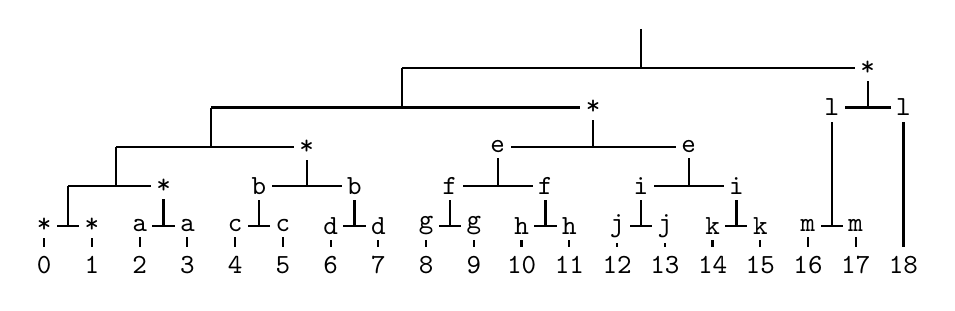
\begin{tikzpicture}[
  x=0.05\textwidth,
  y=1cm,
]
  \coordinate (root) at (12.5, 3.0) {};

  \coordinate(al) at (7.5, 2.5) {};
  \coordinate(ac) at (12.5, 2.5) {};
  \coordinate (ar) at (17.25, 2.5) {};

  \coordinate (bl) at (3.5, 2.0) {};
  \coordinate (bc) at (7.5, 2.0) {};
  \coordinate (br) at (11.5, 2.0) {};
  \coordinate (ql) at (16.5, 2.0) {};
  \coordinate (qc) at (17.25, 2.0) {};
  \coordinate (qr) at (18, 2.0) {};

  \coordinate (cl) at (1.5, 1.5) {};
  \coordinate (cc) at (3.5, 1.5) {};
  \coordinate (cr) at (5.5, 1.5) {};
  \coordinate (jl) at (9.5, 1.5) {};
  \coordinate (jc) at (11.5, 1.5) {};
  \coordinate (jr) at (13.5, 1.5) {};

  \coordinate (dl) at (0.5, 1.0) {};
  \coordinate (dc) at (1.5, 1.0) {};
  \coordinate (dr) at (2.5, 1.0) {};
  \coordinate (gl) at (4.5, 1.0) {};
  \coordinate (gc) at (5.5, 1.0) {};
  \coordinate (gr) at (6.5, 1.0) {};
  \coordinate (kl) at (8.5, 1.0) {};
  \coordinate (kc) at (9.5, 1.0) {};
  \coordinate (kr) at (10.5, 1.0) {};
  \coordinate (nl) at (12.5, 1.0) {};
  \coordinate (nc) at (13.5, 1.0) {};
  \coordinate (nr) at (14.5, 1.0) {};

  \coordinate (el) at (0, 0.5) {};
  \coordinate (ec) at (0.5, 0.5) {};
  \coordinate (er) at (1, 0.5) {};
  \coordinate (fl) at (2, 0.5) {};
  \coordinate (fc) at (2.5, 0.5) {};
  \coordinate (fr) at (3, 0.5) {};
  \coordinate (hl) at (4, 0.5) {};
  \coordinate (hc) at (4.5, 0.5) {};
  \coordinate (hr) at (5, 0.5) {};
  \coordinate (il) at (6, 0.5) {};
  \coordinate (ic) at (6.5, 0.5) {};
  \coordinate (ir) at (7, 0.5) {};
  \coordinate (ll) at (8, 0.5) {};
  \coordinate (lc) at (8.5, 0.5) {};
  \coordinate (lr) at (9, 0.5) {};
  \coordinate (ml) at (10, 0.5) {};
  \coordinate (mc) at (10.5, 0.5) {};
  \coordinate (mr) at (11, 0.5) {};
  \coordinate (ol) at (12, 0.5) {};
  \coordinate (oc) at (12.5, 0.5) {};
  \coordinate (or) at (13, 0.5) {};
  \coordinate (pl) at (14, 0.5) {};
  \coordinate (pc) at (14.5, 0.5) {};
  \coordinate (pr) at (15, 0.5) {};
  \coordinate (rl) at (16, 0.5) {};
  \coordinate (rc) at (16.5, 0.5) {};
  \coordinate (rr) at (17, 0.5) {};

  \node[draw=none] (n0) at (0,0) {\texttt{0}};
  \node[draw=none] (n1) at (1,0) {\texttt{1}};
  \node[draw=none] (n2) at (2,0) {\texttt{2}};
  \node[draw=none] (n3) at (3,0) {\texttt{3}};
  \node[draw=none] (n4) at (4,0) {\texttt{4}};
  \node[draw=none] (n5) at (5,0) {\texttt{5}};
  \node[draw=none] (n6) at (6,0) {\texttt{6}};
  \node[draw=none] (n7) at (7,0) {\texttt{7}};
  \node[draw=none] (n8) at (8,0) {\texttt{8}};
  \node[draw=none] (n9) at (9,0) {\texttt{9}};
  \node[draw=none] (n10) at (10,0) {\texttt{10}};
  \node[draw=none] (n11) at (11,0) {\texttt{11}};
  \node[draw=none] (n12) at (12,0) {\texttt{12}};
  \node[draw=none] (n13) at (13,0) {\texttt{13}};
  \node[draw=none] (n14) at (14,0) {\texttt{14}};
  \node[draw=none] (n15) at (15,0) {\texttt{15}};
  \node[draw=none] (n16) at (16,0) {\texttt{16}};
  \node[draw=none] (n17) at (17,0) {\texttt{17}};
  \node[draw=none] (n18) at (18,0) {\texttt{18}};

  \draw[thick] (root) -| (ac);
  \draw[thick] (ac) -| (al);
  \draw[thick] (al) -| (bc);
  \draw[thick] (ac) -| (ar);
  \draw[thick] (ar) -| (qc);
  \draw[thick] (bc) -| (bl);
  \draw[thick] (bl) -| (cc);
  \draw[thick] (bc) -| (br);
  \draw[thick] (br) -| (jc);
  \draw[thick] (qc) -| (ql);
  \draw[thick] (ql) -| (rc);
  \draw[thick] (qc) -| (qr);
  \draw[thick] (qr) -| (n18);
  \draw[thick] (cc) -| (cl);
  \draw[thick] (cl) -| (dc);
  \draw[thick] (cc) -| (cr);
  \draw[thick] (cr) -| (gc);
  \draw[thick] (jc) -| (jl);
  \draw[thick] (jl) -| (kc);
  \draw[thick] (jc) -| (jr);
  \draw[thick] (jr) -| (nc);
  \draw[thick] (dc) -| (dl);
  \draw[thick] (dl) -| (ec);
  \draw[thick] (dc) -| (dr);
  \draw[thick] (dr) -| (fc);
  \draw[thick] (gc) -| (gl);
  \draw[thick] (gl) -| (hc);
  \draw[thick] (gc) -| (gr);
  \draw[thick] (gr) -| (ic);
  \draw[thick] (kr) -| (kl);
  \draw[thick] (kc) -| (kl);
  \draw[thick] (kl) -| (lc);
  \draw[thick] (kc) -| (kr);
  \draw[thick] (kr) -| (mc);
  \draw[thick] (nc) -| (nl);
  \draw[thick] (nl) -| (oc);
  \draw[thick] (nc) -| (nr);
  \draw[thick] (nr) -| (pc);
  \draw[thick] (ec) -| (el);
  \draw[thick] (el) -| (n0);
  \draw[thick] (ec) -| (er);
  \draw[thick] (er) -| (n1);
  \draw[thick] (fc) -| (fl);
  \draw[thick] (fl) -| (n2);
  \draw[thick] (fc) -| (fr);
  \draw[thick] (fr) -| (n3);
  \draw[thick] (hc) -| (hl);
  \draw[thick] (hl) -| (n4);
  \draw[thick] (hc) -| (hr);
  \draw[thick] (hr) -| (n5);
  \draw[thick] (ic) -| (il);
  \draw[thick] (il) -| (n6);
  \draw[thick] (ic) -| (ir);
  \draw[thick] (ir) -| (n7);
  \draw[thick] (lc) -| (ll);
  \draw[thick] (ll) -| (n8);
  \draw[thick] (lc) -| (lr);
  \draw[thick] (lr) -| (n9);
  \draw[thick] (mc) -| (ml);
  \draw[thick] (ml) -| (n10);
  \draw[thick] (mc) -| (mr);
  \draw[thick] (mr) -| (n11);
  \draw[thick] (oc) -| (ol);
  \draw[thick] (ol) -| (n12);
  \draw[thick] (oc) -| (or);
  \draw[thick] (or) -| (n13);
  \draw[thick] (pc) -| (pl);
  \draw[thick] (pl) -| (n14);
  \draw[thick] (pc) -| (pr);
  \draw[thick] (pr) -| (n15);
  \draw[thick] (rc) -| (rl);
  \draw[thick] (rl) -| (n16);
  \draw[thick] (rc) -| (rr);
  \draw[thick] (rr) -| (n17);

  \node[draw=none, fill=white, inner sep=2pt] at (el) {\texttt{*}};
  \node[draw=none, fill=white, inner sep=2pt] at (er) {\texttt{*}};
  \node[draw=none, fill=white, inner sep=2pt] at (fl) {\texttt{a}};
  \node[draw=none, fill=white, inner sep=2pt] at (fr) {\texttt{a}};
  \node[draw=none, fill=white, inner sep=2pt] at (hl) {\texttt{c}};
  \node[draw=none, fill=white, inner sep=2pt] at (hr) {\texttt{c}};
  \node[draw=none, fill=white, inner sep=2pt] at (il) {\texttt{d}};
  \node[draw=none, fill=white, inner sep=2pt] at (ir) {\texttt{d}};
  \node[draw=none, fill=white, inner sep=2pt] at (ll) {\texttt{g}};
  \node[draw=none, fill=white, inner sep=2pt] at (lr) {\texttt{g}};
  \node[draw=none, fill=white, inner sep=2pt] at (ml) {\texttt{h}};
  \node[draw=none, fill=white, inner sep=2pt] at (mr) {\texttt{h}};
  \node[draw=none, fill=white, inner sep=2pt] at (ol) {\texttt{j}};
  \node[draw=none, fill=white, inner sep=2pt] at (or) {\texttt{j}};
  \node[draw=none, fill=white, inner sep=2pt] at (pl) {\texttt{k}};
  \node[draw=none, fill=white, inner sep=2pt] at (pr) {\texttt{k}};
  \node[draw=none, fill=white, inner sep=2pt] at (rl) {\texttt{m}};
  \node[draw=none, fill=white, inner sep=2pt] at (rr) {\texttt{m}};
  \node[draw=none, fill=white, inner sep=2pt] at (dr) {\texttt{*}};
  \node[draw=none, fill=white, inner sep=2pt] at (cr) {\texttt{*}};
  \node[draw=none, fill=white, inner sep=2pt] at (br) {\texttt{*}};
  \node[draw=none, fill=white, inner sep=2pt] at (ar) {\texttt{*}};
  \node[draw=none, fill=white, inner sep=2pt] at (gl) {\texttt{b}};
  \node[draw=none, fill=white, inner sep=2pt] at (gr) {\texttt{b}};
  \node[draw=none, fill=white, inner sep=2pt] at (kl) {\texttt{f}};
  \node[draw=none, fill=white, inner sep=2pt] at (kr) {\texttt{f}};
  \node[draw=none, fill=white, inner sep=2pt] at (jl) {\texttt{e}};
  \node[draw=none, fill=white, inner sep=2pt] at (jr) {\texttt{e}};
  \node[draw=none, fill=white, inner sep=2pt] at (nl) {\texttt{i}};
  \node[draw=none, fill=white, inner sep=2pt] at (nr) {\texttt{i}};
  \node[draw=none, fill=white, inner sep=2pt] at (ql) {\texttt{l}};
  \node[draw=none, fill=white, inner sep=2pt] at (qr) {\texttt{l}};
\end{tikzpicture}

In the initial packet, we send the Merkle proof for leaf 0, i.\,e.\ all of the hashes marked with \texttt{*}. Each subsequent packet contains leaf data (leaf 0, 1, 2, etc.), and possibly a ``pair'' (\lstinline[style=inlinecode]{a}, \lstinline[style=inlinecode]{b}, \lstinline[style=inlinecode]{c}, etc.), which comprises \emph{both} child hashes under a particular node. Packet-by-packet, the verifier sees:

\begin{lstlisting}[style=listingblock]
Packet 0: Signed Merkle root + Merkle proof for leaf 0.
          Verify proof against signed root.
          We now have [0,1), [1,2), [2,4), [4,8), [8,16), and [16,19).
Packet 1: Leaf 0 + Pair a.
          Verify leaf 0 against [0,1).
          Verify pair a against [2,4).
          We now have [1,2), [2,3), [3,4), [4,8), [8,16), and [16,19).
Packet 2: Leaf 1 + Pair b.
          Verify leaf 1 against [1,2).
          Verify pair b against [4,8).
          We now have [2,3), [3,4), [4,6), [6,8), [8,16), and [16,19).
Packet 3: Leaf 2 + Pair c.
          Verify leaf 2 against [2,3).
          Verify pair c against [4,6).
          We now have [3,4), [4,5), [5,6), [6,8), [8,16), and [16,19).
... and so on.
\end{lstlisting}

At each step, we ``consume'' two hashes (one to verify a leaf, one to verify a pair), and add the pair to our verified set; thus, the number of verified-but-unused hashes stays constant until we get to packet 13. At this point, packets still contain leaf data (so we'll consume one hash), but there are no more pairs left to send; thus, our stockpile of hashes is steadily exhausted, until we consume the final hash to verify the final packet.

This is a solid improvement! We dubbed it ``Lockstep Streaming,'' after the fact that verification proceeds in lockstep with packet receipt. But when we sat down to write the code for matching verified-but-unused hashes to incoming leaves and pairs, things got hairy. It was clearly \emph{possible}, but the ugliness of the logic suggested that there was a better way. And after filling plenty of notebook pages with hand-drawn Merkle trees, \patp{rovnys-ricfer} found it: a mapping of packet numbers to hash pairs that was not only much cleaner, but also \emph{scale invariant}. It's called Blackman ordering, and it looks like this:

%                        ┌──────────────┴─────────────*
%            ┌───────────┴───────────*              h─┴─h
%      ┌─────┴─────*           d─────┴─────d        │   │
%   ┌──┴──*     b──┴──b     f──┴──f     j──┴──j     │   │
% *─┴─* a─┴─a c─┴─c e─┴─e g─┴─g i─┴─i k─┴─k m─┴─m o─┴─o │
% 0   1 2   3 4   5 6   7 8   9 10 11 12 13 14 15 16 17 18

\noindent
\hspace{3pt}
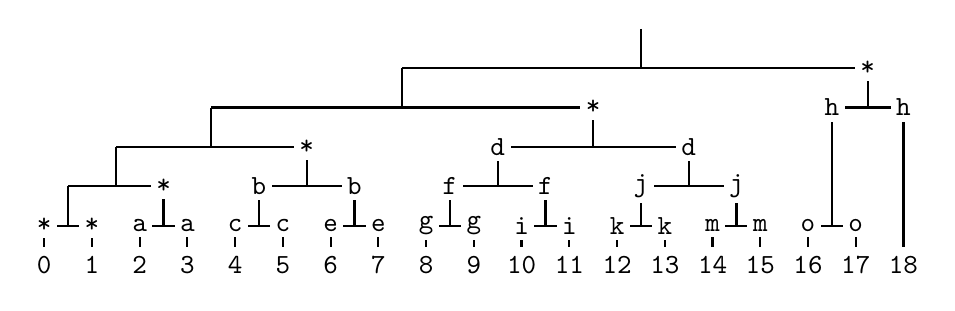
\begin{tikzpicture}[
  x=0.05\textwidth,
  y=1cm,
]
  \coordinate (root) at (12.5, 3.0) {};

  \coordinate(al) at (7.5, 2.5) {};
  \coordinate(ac) at (12.5, 2.5) {};
  \coordinate (ar) at (17.25, 2.5) {};

  \coordinate (bl) at (3.5, 2.0) {};
  \coordinate (bc) at (7.5, 2.0) {};
  \coordinate (br) at (11.5, 2.0) {};
  \coordinate (ql) at (16.5, 2.0) {};
  \coordinate (qc) at (17.25, 2.0) {};
  \coordinate (qr) at (18, 2.0) {};

  \coordinate (cl) at (1.5, 1.5) {};
  \coordinate (cc) at (3.5, 1.5) {};
  \coordinate (cr) at (5.5, 1.5) {};
  \coordinate (jl) at (9.5, 1.5) {};
  \coordinate (jc) at (11.5, 1.5) {};
  \coordinate (jr) at (13.5, 1.5) {};

  \coordinate (dl) at (0.5, 1.0) {};
  \coordinate (dc) at (1.5, 1.0) {};
  \coordinate (dr) at (2.5, 1.0) {};
  \coordinate (gl) at (4.5, 1.0) {};
  \coordinate (gc) at (5.5, 1.0) {};
  \coordinate (gr) at (6.5, 1.0) {};
  \coordinate (kl) at (8.5, 1.0) {};
  \coordinate (kc) at (9.5, 1.0) {};
  \coordinate (kr) at (10.5, 1.0) {};
  \coordinate (nl) at (12.5, 1.0) {};
  \coordinate (nc) at (13.5, 1.0) {};
  \coordinate (nr) at (14.5, 1.0) {};

  \coordinate (el) at (0, 0.5) {};
  \coordinate (ec) at (0.5, 0.5) {};
  \coordinate (er) at (1, 0.5) {};
  \coordinate (fl) at (2, 0.5) {};
  \coordinate (fc) at (2.5, 0.5) {};
  \coordinate (fr) at (3, 0.5) {};
  \coordinate (hl) at (4, 0.5) {};
  \coordinate (hc) at (4.5, 0.5) {};
  \coordinate (hr) at (5, 0.5) {};
  \coordinate (il) at (6, 0.5) {};
  \coordinate (ic) at (6.5, 0.5) {};
  \coordinate (ir) at (7, 0.5) {};
  \coordinate (ll) at (8, 0.5) {};
  \coordinate (lc) at (8.5, 0.5) {};
  \coordinate (lr) at (9, 0.5) {};
  \coordinate (ml) at (10, 0.5) {};
  \coordinate (mc) at (10.5, 0.5) {};
  \coordinate (mr) at (11, 0.5) {};
  \coordinate (ol) at (12, 0.5) {};
  \coordinate (oc) at (12.5, 0.5) {};
  \coordinate (or) at (13, 0.5) {};
  \coordinate (pl) at (14, 0.5) {};
  \coordinate (pc) at (14.5, 0.5) {};
  \coordinate (pr) at (15, 0.5) {};
  \coordinate (rl) at (16, 0.5) {};
  \coordinate (rc) at (16.5, 0.5) {};
  \coordinate (rr) at (17, 0.5) {};

  \node[draw=none] (n0) at (0,0) {\texttt{0}};
  \node[draw=none] (n1) at (1,0) {\texttt{1}};
  \node[draw=none] (n2) at (2,0) {\texttt{2}};
  \node[draw=none] (n3) at (3,0) {\texttt{3}};
  \node[draw=none] (n4) at (4,0) {\texttt{4}};
  \node[draw=none] (n5) at (5,0) {\texttt{5}};
  \node[draw=none] (n6) at (6,0) {\texttt{6}};
  \node[draw=none] (n7) at (7,0) {\texttt{7}};
  \node[draw=none] (n8) at (8,0) {\texttt{8}};
  \node[draw=none] (n9) at (9,0) {\texttt{9}};
  \node[draw=none] (n10) at (10,0) {\texttt{10}};
  \node[draw=none] (n11) at (11,0) {\texttt{11}};
  \node[draw=none] (n12) at (12,0) {\texttt{12}};
  \node[draw=none] (n13) at (13,0) {\texttt{13}};
  \node[draw=none] (n14) at (14,0) {\texttt{14}};
  \node[draw=none] (n15) at (15,0) {\texttt{15}};
  \node[draw=none] (n16) at (16,0) {\texttt{16}};
  \node[draw=none] (n17) at (17,0) {\texttt{17}};
  \node[draw=none] (n18) at (18,0) {\texttt{18}};

  \draw[thick] (root) -| (ac);
  \draw[thick] (ac) -| (al);
  \draw[thick] (al) -| (bc);
  \draw[thick] (ac) -| (ar);
  \draw[thick] (ar) -| (qc);
  \draw[thick] (bc) -| (bl);
  \draw[thick] (bl) -| (cc);
  \draw[thick] (bc) -| (br);
  \draw[thick] (br) -| (jc);
  \draw[thick] (qc) -| (ql);
  \draw[thick] (ql) -| (rc);
  \draw[thick] (qc) -| (qr);
  \draw[thick] (qr) -| (n18);
  \draw[thick] (cc) -| (cl);
  \draw[thick] (cl) -| (dc);
  \draw[thick] (cc) -| (cr);
  \draw[thick] (cr) -| (gc);
  \draw[thick] (jc) -| (jl);
  \draw[thick] (jl) -| (kc);
  \draw[thick] (jc) -| (jr);
  \draw[thick] (jr) -| (nc);
  \draw[thick] (dc) -| (dl);
  \draw[thick] (dl) -| (ec);
  \draw[thick] (dc) -| (dr);
  \draw[thick] (dr) -| (fc);
  \draw[thick] (gc) -| (gl);
  \draw[thick] (gl) -| (hc);
  \draw[thick] (gc) -| (gr);
  \draw[thick] (gr) -| (ic);
  \draw[thick] (kr) -| (kl);
  \draw[thick] (kc) -| (kl);
  \draw[thick] (kl) -| (lc);
  \draw[thick] (kc) -| (kr);
  \draw[thick] (kr) -| (mc);
  \draw[thick] (nc) -| (nl);
  \draw[thick] (nl) -| (oc);
  \draw[thick] (nc) -| (nr);
  \draw[thick] (nr) -| (pc);
  \draw[thick] (ec) -| (el);
  \draw[thick] (el) -| (n0);
  \draw[thick] (ec) -| (er);
  \draw[thick] (er) -| (n1);
  \draw[thick] (fc) -| (fl);
  \draw[thick] (fl) -| (n2);
  \draw[thick] (fc) -| (fr);
  \draw[thick] (fr) -| (n3);
  \draw[thick] (hc) -| (hl);
  \draw[thick] (hl) -| (n4);
  \draw[thick] (hc) -| (hr);
  \draw[thick] (hr) -| (n5);
  \draw[thick] (ic) -| (il);
  \draw[thick] (il) -| (n6);
  \draw[thick] (ic) -| (ir);
  \draw[thick] (ir) -| (n7);
  \draw[thick] (lc) -| (ll);
  \draw[thick] (ll) -| (n8);
  \draw[thick] (lc) -| (lr);
  \draw[thick] (lr) -| (n9);
  \draw[thick] (mc) -| (ml);
  \draw[thick] (ml) -| (n10);
  \draw[thick] (mc) -| (mr);
  \draw[thick] (mr) -| (n11);
  \draw[thick] (oc) -| (ol);
  \draw[thick] (ol) -| (n12);
  \draw[thick] (oc) -| (or);
  \draw[thick] (or) -| (n13);
  \draw[thick] (pc) -| (pl);
  \draw[thick] (pl) -| (n14);
  \draw[thick] (pc) -| (pr);
  \draw[thick] (pr) -| (n15);
  \draw[thick] (rc) -| (rl);
  \draw[thick] (rl) -| (n16);
  \draw[thick] (rc) -| (rr);
  \draw[thick] (rr) -| (n17);

  \node[draw=none, fill=white, inner sep=2pt] at (el) {\texttt{*}};
  \node[draw=none, fill=white, inner sep=2pt] at (er) {\texttt{*}};
  \node[draw=none, fill=white, inner sep=2pt] at (fl) {\texttt{a}};
  \node[draw=none, fill=white, inner sep=2pt] at (fr) {\texttt{a}};
  \node[draw=none, fill=white, inner sep=2pt] at (hl) {\texttt{c}};
  \node[draw=none, fill=white, inner sep=2pt] at (hr) {\texttt{c}};
  \node[draw=none, fill=white, inner sep=2pt] at (il) {\texttt{e}};
  \node[draw=none, fill=white, inner sep=2pt] at (ir) {\texttt{e}};
  \node[draw=none, fill=white, inner sep=2pt] at (ll) {\texttt{g}};
  \node[draw=none, fill=white, inner sep=2pt] at (lr) {\texttt{g}};
  \node[draw=none, fill=white, inner sep=2pt] at (ml) {\texttt{i}};
  \node[draw=none, fill=white, inner sep=2pt] at (mr) {\texttt{i}};
  \node[draw=none, fill=white, inner sep=2pt] at (ol) {\texttt{k}};
  \node[draw=none, fill=white, inner sep=2pt] at (or) {\texttt{k}};
  \node[draw=none, fill=white, inner sep=2pt] at (pl) {\texttt{m}};
  \node[draw=none, fill=white, inner sep=2pt] at (pr) {\texttt{m}};
  \node[draw=none, fill=white, inner sep=2pt] at (rl) {\texttt{o}};
  \node[draw=none, fill=white, inner sep=2pt] at (rr) {\texttt{o}};
  \node[draw=none, fill=white, inner sep=2pt] at (dr) {\texttt{*}};
  \node[draw=none, fill=white, inner sep=2pt] at (cr) {\texttt{*}};
  \node[draw=none, fill=white, inner sep=2pt] at (br) {\texttt{*}};
  \node[draw=none, fill=white, inner sep=2pt] at (ar) {\texttt{*}};
  \node[draw=none, fill=white, inner sep=2pt] at (gl) {\texttt{b}};
  \node[draw=none, fill=white, inner sep=2pt] at (gr) {\texttt{b}};
  \node[draw=none, fill=white, inner sep=2pt] at (kl) {\texttt{f}};
  \node[draw=none, fill=white, inner sep=2pt] at (kr) {\texttt{f}};
  \node[draw=none, fill=white, inner sep=2pt] at (jl) {\texttt{d}};
  \node[draw=none, fill=white, inner sep=2pt] at (jr) {\texttt{d}};
  \node[draw=none, fill=white, inner sep=2pt] at (nl) {\texttt{j}};
  \node[draw=none, fill=white, inner sep=2pt] at (nr) {\texttt{j}};
  \node[draw=none, fill=white, inner sep=2pt] at (ql) {\texttt{h}};
  \node[draw=none, fill=white, inner sep=2pt] at (qr) {\texttt{h}};
\end{tikzpicture}

See the difference? Instead of ordering the pairs on a first-needed basis, we jump around a bit. Specifically, we send a pair whose ``height'' corresponds to the number of trailing zeroes in the binary representation of the packet number. For example, packet 4 is \lstinline[style=inlinecode]{0b100} in binary, with two trailing zeroes, so we send pair d, which sits two levels above the leaves.\footnote{As you might expect, the logic gets slightly less clean when the number of leaves is not a power of two, but it's hardly catastrophic.} Here is a packet-by-packet verification for Blackman ordering:

The \lstinline[style=inlinecode]{[x,y)} notation indicates a half-open set, i.\,e.\ it includes \lstinline[style=inlinecode]{x}, \lstinline[style=inlinecode]{x+1}, \lstinline[style=inlinecode]{x+2}, \ldots{}, \lstinline[style=inlinecode]{y-1}.  \lstinline[style=inlinecode]{[2,4)} contains elements \lstinline[style=inlinecode]{2} and \lstinline[style=inlinecode]{3}.  \lstinline[style=inlinecode]{[0,1)} contains the single element \lstinline[style=inlinecode]{0}.

\begin{lstlisting}[style=listingblock]
Packet 0: Signed Merkle root + Merkle proof for leaf 0.
          Verify proof against signed root.
          We now have [0,1), [1,2), [2,4), [4,8), [8,16), and [16,19).

Packet 1: Leaf 0 + Pair a.
          Verify leaf 0 against [0,1).
          Verify pair a against [2,4).
          We now have [1,2), [2,3), [3,4), [4,8), [8,16), and [16,19).
Packet 2: Leaf 1 + Pair b.
          Verify leaf 1 against [1,2).
          Verify pair b against [4,8).
          We now have [2,3), [3,4), [4,6), [6,8), [8,16), and [16,19).
Packet 3: Leaf 2 + Pair c.
          Verify leaf 2 against [2,3).
          Verify pair c against [4,6).
          We now have [3,4), [4,5), [5,6), [6,8), [8,16), and [16,19).
... and so on.
\end{lstlisting}

Shortly after, \patp{watter-parter} tweaked the ordering slightly, offsetting it by one; this further simplified the low-level bithacking. We called this variant ``Lackman ordering,'' and it is used in the final version of Lockstep Streaming.  A diagram of the order is depicted in Figure~\ref{fig:lackman-1}.

Per-packet verification for Lackman ordering looks like:

\begin{lstlisting}[style=listingblock]
Packet 0: Signed Merkle root + Merkle proof for leaf 0.
          Verify proof against signed root.
          We now have [0,1), [1,2), [2,4), [4,8), [8,16), and [16,19).
Packet 1: Leaf 0 (no pair).
          Verify leaf 0 against [0,1).
          We now have [1,2), [2,4), [4,8), [8,16), and [16,19).
Packet 2: Leaf 1 + Pair a.
          Verify leaf 1 against [1,2).
          Verify pair a against [2,4).
          We now have [2,3), [3,4), [4,8), [8,16), and [16,19).
Packet 3: Leaf 2 + Pair b.
          Verify leaf 2 against [2,3).
          Verify pair b against [4,8).
          We now have [3,4), [4,6), [6,8), [8,16), and [16,19).
... and so on.
\end{lstlisting}

\begin{figure}[htbp]
  \centering
  \begin{subfigure}{\textwidth}
    \centering
    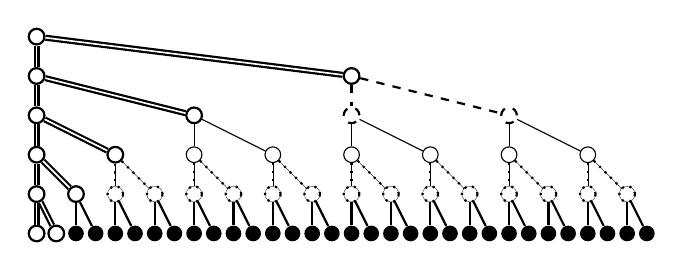
\begin{tikzpicture}[align=center]
      \node[draw=black, thick, fill=white, circle, inner sep=2pt] (T1) at (0,2.5) {};
      %
      \node[draw=black, thick, fill=white, circle, inner sep=2pt] (U2) at (0,2) {};
      \node[draw=black, thick, fill=white, circle, inner sep=2pt] (U3) at (4,2) {};
      %
      \node[draw=black, thick, fill=white, circle, inner sep=2pt] (V4) at (0,1.5) {};
      \node[draw=black, thick, fill=white, circle, inner sep=2pt] (V5) at (2,1.5) {};
      \node[draw=black, thick, dashed, fill=white, circle, inner sep=2pt] (V6) at (4,1.5) {};
      \node[draw=black, thick, dashed, fill=white, circle, inner sep=2pt] (V7) at (6,1.5) {};
      %
      \node[draw=black, thick, fill=white, circle, inner sep=2pt] (W8) at (0,1) {};
      \node[draw=black, thick, fill=white, circle, inner sep=2pt] (W9) at (1,1) {};
      \node[draw=black, circle, inner sep=2pt] (W10) at (2,1) {};
      \node[draw=black, circle, inner sep=2pt] (W11) at (3,1) {};
      \node[draw=black, circle, inner sep=2pt] (W12) at (4,1) {};
      \node[draw=black, circle, inner sep=2pt] (W13) at (5,1) {};
      \node[draw=black, circle, inner sep=2pt] (W14) at (6,1) {};
      \node[draw=black, circle, inner sep=2pt] (W15) at (7,1) {};
      %
      \node[draw=black, thick, fill=white, circle, inner sep=2pt] (X16) at (0,0.5) {};
      \node[draw=black, thick, fill=white, circle, inner sep=2pt] (X17) at (0.5,0.5) {};
      \node[draw=black, thick, dotted, fill=white, circle, inner sep=2pt] (X18) at (1,0.5) {};
      \node[draw=black, ultra thin, circle, inner sep=2pt] (X18) at (1,0.5) {};
      %
      \node[draw=black, thick, dotted, fill=white, circle, inner sep=2pt] (X19) at (1.5,0.5) {};
      \node[draw=black, ultra thin, circle, inner sep=2pt] (X19) at (1.5,0.5) {};
      %
      \node[draw=black, thick, dotted, fill=white, circle, inner sep=2pt] (X20) at (2,0.5) {};
      \node[draw=black, ultra thin, circle, inner sep=2pt] (X20) at (2,0.5) {};
      %
      \node[draw=black, thick, dotted, fill=white, circle, inner sep=2pt] (X21) at (2.5,0.5) {};
      \node[draw=black, ultra thin, circle, inner sep=2pt] (X21) at (2.5,0.5) {};
      %
      \node[draw=black, thick, dotted, fill=white, circle, inner sep=2pt] (X22) at (3,0.5) {};
      \node[draw=black, ultra thin, circle, inner sep=2pt] (X22) at (3,0.5) {};
      %
      \node[draw=black, thick, dotted, fill=white, circle, inner sep=2pt] (X23) at (3.5,0.5) {};
      \node[draw=black, ultra thin, circle, inner sep=2pt] (X23) at (3.5,0.5) {};
      %
      \node[draw=black, thick, dotted, fill=white, circle, inner sep=2pt] (X24) at (4,0.5) {};
      \node[draw=black, ultra thin, circle, inner sep=2pt] (X24) at (4,0.5) {};
      %
      \node[draw=black, thick, dotted, fill=white, circle, inner sep=2pt] (X25) at (4.5,0.5) {};
      \node[draw=black, ultra thin, circle, inner sep=2pt] (X25) at (4.5,0.5) {};
      %
      \node[draw=black, thick, dotted, fill=white, circle, inner sep=2pt] (X26) at (5,0.5) {};
      \node[draw=black, ultra thin, circle, inner sep=2pt] (X26) at (5,0.5) {};
      %
      \node[draw=black, thick, dotted, fill=white, circle, inner sep=2pt] (X27) at (5.5,0.5) {};
      \node[draw=black, ultra thin, circle, inner sep=2pt] (X27) at (5.5,0.5) {};
      %
      \node[draw=black, thick, dotted, fill=white, circle, inner sep=2pt] (X28) at (6,0.5) {};
      \node[draw=black, ultra thin, circle, inner sep=2pt] (X28) at (6,0.5) {};
      %
      \node[draw=black, thick, dotted, fill=white, circle, inner sep=2pt] (X29) at (6.5,0.5) {};
      \node[draw=black, ultra thin, circle, inner sep=2pt] (X29) at (6.5,0.5) {};
      %
      \node[draw=black, thick, dotted, fill=white, circle, inner sep=2pt] (X30) at (7,0.5) {};
      \node[draw=black, ultra thin, circle, inner sep=2pt] (X30) at (7,0.5) {};
      %
      \node[draw=black, thick, dotted, fill=white, circle, inner sep=2pt] (X31) at (7.5,0.5) {};
      \node[draw=black, ultra thin, circle, inner sep=2pt] (X31) at (7.5,0.5) {};
      %
      \node[draw=black, thick, fill=white, circle, inner sep=2pt] (Y32) at (0,0) {};
      \node[draw=black, thick, fill=white, circle, inner sep=2pt] (Y33) at (0.25,0) {};
      \node[fill=black, circle, inner sep=2pt] (Y34) at (0.5,0) {};
      \node[fill=black, circle, inner sep=2pt] (Y35) at (0.75,0) {};
      \node[fill=black, circle, inner sep=2pt] (Y36) at (1,0) {};
      \node[fill=black, circle, inner sep=2pt] (Y37) at (1.25,0) {};
      \node[fill=black, circle, inner sep=2pt] (Y38) at (1.5,0) {};
      \node[fill=black, circle, inner sep=2pt] (Y39) at (1.75,0) {};
      \node[fill=black, circle, inner sep=2pt] (Y40) at (2,0) {};
      \node[fill=black, circle, inner sep=2pt] (Y41) at (2.25,0) {};
      \node[fill=black, circle, inner sep=2pt] (Y42) at (2.5,0) {};
      \node[fill=black, circle, inner sep=2pt] (Y43) at (2.75,0) {};
      \node[fill=black, circle, inner sep=2pt] (Y44) at (3,0) {};
      \node[fill=black, circle, inner sep=2pt] (Y45) at (3.25,0) {};
      \node[fill=black, circle, inner sep=2pt] (Y46) at (3.5,0) {};
      \node[fill=black, circle, inner sep=2pt] (Y47) at (3.75,0) {};
      \node[fill=black, circle, inner sep=2pt] (Y48) at (4,0) {};
      \node[fill=black, circle, inner sep=2pt] (Y49) at (4.25,0) {};
      \node[fill=black, circle, inner sep=2pt] (Y50) at (4.5,0) {};
      \node[fill=black, circle, inner sep=2pt] (Y51) at (4.75,0) {};
      \node[fill=black, circle, inner sep=2pt] (Y52) at (5,0) {};
      \node[fill=black, circle, inner sep=2pt] (Y53) at (5.25,0) {};
      \node[fill=black, circle, inner sep=2pt] (Y54) at (5.5,0) {};
      \node[fill=black, circle, inner sep=2pt] (Y55) at (5.75,0) {};
      \node[fill=black, circle, inner sep=2pt] (Y56) at (6,0) {};
      \node[fill=black, circle, inner sep=2pt] (Y57) at (6.25,0) {};
      \node[fill=black, circle, inner sep=2pt] (Y58) at (6.5,0) {};
      \node[fill=black, circle, inner sep=2pt] (Y59) at (6.75,0) {};
      \node[fill=black, circle, inner sep=2pt] (Y60) at (7,0) {};
      \node[fill=black, circle, inner sep=2pt] (Y61) at (7.25,0) {};
      \node[fill=black, circle, inner sep=2pt] (Y62) at (7.5,0) {};
      \node[fill=black, circle, inner sep=2pt] (Y63) at (7.75,0) {};
      %
      \draw[thick, double] (T1) -- (U2);
      \draw[thick, double] (T1) -- (U3);
      %
      \draw[thick, double] (U2) -- (V4);
      \draw[thick, double] (U2) -- (V5);
      \draw[thick, dashed] (U3) -- (V6);
      \draw[thick, dashed] (U3) -- (V7);
      %
      \draw[thick, double] (V4) -- (W8);
      \draw[thick, double] (V4) -- (W9);
      \draw[] (V5) -- (W10);
      \draw[] (V5) -- (W11);
      \draw[] (V6) -- (W12);
      \draw[] (V6) -- (W13);
      \draw[] (V7) -- (W14);
      \draw[] (V7) -- (W15);
      %
      \draw[thick, double] (W8) -- (X16);
      \draw[thick, double] (W8) -- (X17);
      \draw[thick, dotted] (W9) -- (X18);
      \draw[ultra thin] (W9) -- (X18);
      \draw[thick, dotted] (W9) -- (X19);
      \draw[ultra thin] (W9) -- (X19);
      \draw[thick, dotted] (W10) -- (X20);
      \draw[ultra thin] (W10) -- (X20);
      \draw[thick, dotted] (W10) -- (X21);
      \draw[ultra thin] (W10) -- (X21);
      \draw[thick, dotted] (W11) -- (X22);
      \draw[ultra thin] (W11) -- (X22);
      \draw[thick, dotted] (W11) -- (X23);
      \draw[ultra thin] (W11) -- (X23);
      \draw[thick, dotted] (W12) -- (X24);
      \draw[ultra thin] (W12) -- (X24);
      \draw[thick, dotted] (W12) -- (X25);
      \draw[ultra thin] (W12) -- (X25);
      \draw[thick, dotted] (W13) -- (X26);
      \draw[ultra thin] (W13) -- (X26);
      \draw[thick, dotted] (W13) -- (X27);
      \draw[ultra thin] (W13) -- (X27);
      \draw[thick, dotted] (W14) -- (X28);
      \draw[ultra thin] (W14) -- (X28);
      \draw[thick, dotted] (W14) -- (X29);
      \draw[ultra thin] (W14) -- (X29);
      \draw[thick, dotted] (W15) -- (X30);
      \draw[ultra thin] (W15) -- (X30);
      \draw[thick, dotted] (W15) -- (X31);
      \draw[ultra thin] (W15) -- (X31);
      %
      \draw[thick, double] (X16) -- (Y32);
      \draw[thick, double] (X16) -- (Y33);
      \draw[thick] (X17) -- (Y34);
      \draw[thick] (X17) -- (Y35);
      \draw[thick] (X18) -- (Y36);
      \draw[thick] (X18) -- (Y37);
      \draw[thick] (X19) -- (Y38);
      \draw[thick] (X19) -- (Y39);
      \draw[thick] (X20) -- (Y40);
      \draw[thick] (X20) -- (Y41);
      \draw[thick] (X21) -- (Y42);
      \draw[thick] (X21) -- (Y43);
      \draw[thick] (X22) -- (Y44);
      \draw[thick] (X22) -- (Y45);
      \draw[thick] (X23) -- (Y46);
      \draw[thick] (X23) -- (Y47);
      \draw[thick] (X24) -- (Y48);
      \draw[thick] (X24) -- (Y49);
      \draw[thick] (X25) -- (Y50);
      \draw[thick] (X25) -- (Y51);
      \draw[thick] (X26) -- (Y52);
      \draw[thick] (X26) -- (Y53);
      \draw[thick] (X27) -- (Y54);
      \draw[thick] (X27) -- (Y55);
      \draw[thick] (X28) -- (Y56);
      \draw[thick] (X28) -- (Y57);
      \draw[thick] (X29) -- (Y58);
      \draw[thick] (X29) -- (Y59);
      \draw[thick] (X30) -- (Y60);
      \draw[thick] (X30) -- (Y61);
      \draw[thick] (X31) -- (Y62);
      \draw[thick] (X31) -- (Y63);
    \end{tikzpicture}
  \end{subfigure}
  \begin{subfigure}{\textwidth}
    \vspace{0.25cm}
    \centering
    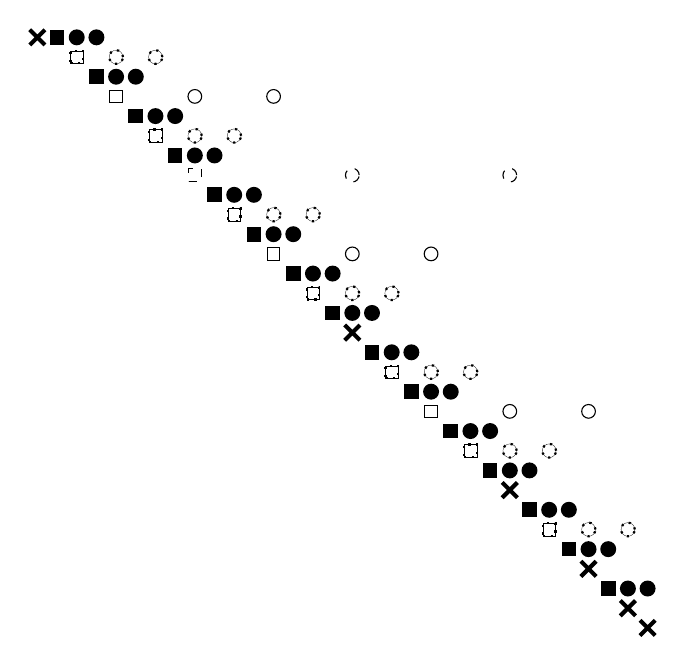
\begin{tikzpicture}[align=center]
      \node[draw=black, line width=1.5pt, fill=black, cross out, inner sep=2pt] (T1) at (0,15.5) {};
      \node[draw=black, thick, fill=black, rectangle, inner sep=2.25pt] (T1) at (0.25,15.5) {};
      \node[draw=black, thick, fill=black, circle, inner sep=1.75pt] (T1) at (0.5,15.5) {};
      \node[draw=black, thick, fill=black, circle, inner sep=1.75pt] (T1) at (0.75,15.5) {};
      %
      \node[draw=black, thick, dotted, fill=white, rectangle, inner sep=2.25pt] (T1) at (0.5,15.25) {};
      \node[draw=black, ultra thin, rectangle, inner sep=2.25pt] (T1) at (0.5,15.25) {};
      \node[draw=black, thick, dotted, fill=white, circle, inner sep=1.75pt] (T1) at (1.0,15.25) {};
      \node[draw=black, ultra thin, circle, inner sep=1.75pt] (T1) at (1.0,15.25) {};
      \node[draw=black, thick, dotted, fill=white, circle, inner sep=1.75pt] (T1) at (1.5,15.25) {};
      \node[draw=black, ultra thin, circle, inner sep=1.75pt] (T1) at (1.5,15.25) {};
      %
      \node[draw=black, thick, fill=black, rectangle, inner sep=2.25pt] (T1) at (0.75,15) {};
      \node[draw=black, thick, fill=black, circle, inner sep=1.75pt] (T1) at (1.0,15) {};
      \node[draw=black, thick, fill=black, circle, inner sep=1.75pt] (T1) at (1.25,15) {};
      %
      \node[draw=black, fill=white, rectangle, inner sep=2.25pt] (T1) at (1,14.75) {};
      \node[draw=black, fill=white, circle, inner sep=1.75pt] (T1) at (2,14.75) {};
      \node[draw=black, fill=white, circle, inner sep=1.75pt] (T1) at (3,14.75) {};
      %
      \node[draw=black, thick, fill=black, rectangle, inner sep=2.25pt] (T1) at (1.25,14.5) {};
      \node[draw=black, thick, fill=black, circle, inner sep=1.75pt] (T1) at (1.5,14.5) {};
      \node[draw=black, thick, fill=black, circle, inner sep=1.75pt] (T1) at (1.75,14.5) {};
      %
      \node[draw=black, thick, dotted, fill=white, rectangle, inner sep=2.25pt] (T1) at (1.5,14.25) {};
      \node[draw=black, ultra thin, rectangle, inner sep=2.25pt] (T1) at (1.5,14.25) {};
      \node[draw=black, thick, dotted, fill=white, circle, inner sep=1.75pt] (T1) at (2,14.25) {};
      \node[draw=black, ultra thin, circle, inner sep=1.75pt] (T1) at (2,14.25) {};
      \node[draw=black, thick, dotted, fill=white, circle, inner sep=1.75pt] (T1) at (2.5,14.25) {};
      \node[draw=black, ultra thin, circle, inner sep=1.75pt] (T1) at (2.5,14.25) {};
      %
      \node[draw=black, thick, fill=black, rectangle, inner sep=2.25pt] (T1) at (1.75,14) {};
      \node[draw=black, thick, fill=black, circle, inner sep=1.75pt] (T1) at (2,14) {};
      \node[draw=black, thick, fill=black, circle, inner sep=1.75pt] (T1) at (2.25,14) {};
      %
      \node[draw=black, dashed, fill=white, rectangle, inner sep=2.25pt] (T1) at (2,13.75) {};
      \node[draw=black, dashed, fill=white, circle, inner sep=1.75pt] (T1) at (4,13.75) {};
      \node[draw=black, dashed, fill=white, circle, inner sep=1.75pt] (T1) at (6,13.75) {};
      %
      \node[draw=black, thick, fill=black, rectangle, inner sep=2.25pt] (T1) at (2.25,13.5) {};
      \node[draw=black, thick, fill=black, circle, inner sep=1.75pt] (T1) at (2.5,13.5) {};
      \node[draw=black, thick, fill=black, circle, inner sep=1.75pt] (T1) at (2.75,13.5) {};
      %
      \node[draw=black, thick, dotted, fill=white, rectangle, inner sep=2.25pt] (T1) at (2.5,13.25) {};
      \node[draw=black, ultra thin, rectangle, inner sep=2.25pt] (T1) at (2.5,13.25) {};
      \node[draw=black, thick, dotted, fill=white, circle, inner sep=1.75pt] (T1) at (3,13.25) {};
      \node[draw=black, ultra thin, circle, inner sep=1.75pt] (T1) at (3,13.25) {};
      \node[draw=black, thick, dotted, fill=white, circle, inner sep=1.75pt] (T1) at (3.5,13.25) {};
      \node[draw=black, ultra thin, circle, inner sep=1.75pt] (T1) at (3.5,13.25) {};
      %
      \node[draw=black, thick, fill=black, rectangle, inner sep=2.25pt] (T1) at (2.75,13) {};
      \node[draw=black, thick, fill=black, circle, inner sep=1.75pt] (T1) at (3,13) {};
      \node[draw=black, thick, fill=black, circle, inner sep=1.75pt] (T1) at (3.25,13) {};
      %
      \node[draw=black, fill=white, rectangle, inner sep=2.25pt] (T1) at (3,12.75) {};
      \node[draw=black, fill=white, circle, inner sep=1.75pt] (T1) at (4,12.75) {};
      \node[draw=black, fill=white, circle, inner sep=1.75pt] (T1) at (5,12.75) {};
      %
      \node[draw=black, thick, fill=black, rectangle, inner sep=2.25pt] (T1) at (3.25,12.5) {};
      \node[draw=black, thick, fill=black, circle, inner sep=1.75pt] (T1) at (3.5,12.5) {};
      \node[draw=black, thick, fill=black, circle, inner sep=1.75pt] (T1) at (3.75,12.5) {};
      %
      \node[draw=black, thick, dotted, fill=white, rectangle, inner sep=2.25pt] (T1) at (3.5,12.25) {};
      \node[draw=black, ultra thin, rectangle, inner sep=2.25pt] (T1) at (3.5,12.25) {};
      \node[draw=black, thick, dotted, fill=white, circle, inner sep=1.75pt] (T1) at (4,12.25) {};
      \node[draw=black, ultra thin, circle, inner sep=1.75pt] (T1) at (4,12.25) {};
      \node[draw=black, thick, dotted, fill=white, circle, inner sep=1.75pt] (T1) at (4.5,12.25) {};
      \node[draw=black, ultra thin, circle, inner sep=1.75pt] (T1) at (4.5,12.25) {};
      %
      \node[draw=black, thick, fill=black, rectangle, inner sep=2.25pt] (T1) at (3.75,12) {};
      \node[draw=black, thick, fill=black, circle, inner sep=1.75pt] (T1) at (4,12) {};
      \node[draw=black, thick, fill=black, circle, inner sep=1.75pt] (T1) at (4.25,12) {};
      %
      \node[draw=black, line width=1.5pt, fill=black, cross out, inner sep=2pt] (T1) at (4,11.75) {};
      %
      \node[draw=black, thick, fill=black, rectangle, inner sep=2.25pt] (T1) at (4.25,11.5) {};
      \node[draw=black, thick, fill=black, circle, inner sep=1.75pt] (T1) at (4.5,11.5) {};
      \node[draw=black, thick, fill=black, circle, inner sep=1.75pt] (T1) at (4.75,11.5) {};
      %
      \node[draw=black, thick, dotted, fill=white, rectangle, inner sep=2.25pt] (T1) at (4.5,11.25) {};
      \node[draw=black, ultra thin, rectangle, inner sep=2.25pt] (T1) at (4.5,11.25) {};
      \node[draw=black, thick, dotted, fill=white, circle, inner sep=1.75pt] (T1) at (5,11.25) {};
      \node[draw=black, ultra thin, circle, inner sep=1.75pt] (T1) at (5,11.25) {};
      \node[draw=black, thick, dotted, fill=white, circle, inner sep=1.75pt] (T1) at (5.5,11.25) {};
      \node[draw=black, ultra thin, circle, inner sep=1.75pt] (T1) at (5.5,11.25) {};
      %
      \node[draw=black, thick, fill=black, rectangle, inner sep=2.25pt] (T1) at (4.75,11) {};
      \node[draw=black, thick, fill=black, circle, inner sep=1.75pt] (T1) at (5,11) {};
      \node[draw=black, thick, fill=black, circle, inner sep=1.75pt] (T1) at (5.25,11) {};
      %
      \node[draw=black, fill=white, rectangle, inner sep=2.25pt] (T1) at (5,10.75) {};
      \node[draw=black, fill=white, circle, inner sep=1.75pt] (T1) at (6,10.75) {};
      \node[draw=black, fill=white, circle, inner sep=1.75pt] (T1) at (7,10.75) {};
      %
      \node[draw=black, thick, fill=black, rectangle, inner sep=2.25pt] (T1) at (5.25,10.5) {};
      \node[draw=black, thick, fill=black, circle, inner sep=1.75pt] (T1) at (5.5,10.5) {};
      \node[draw=black, thick, fill=black, circle, inner sep=1.75pt] (T1) at (5.75,10.5) {};
      %
      \node[draw=black, thick, dotted, fill=white, rectangle, inner sep=2.25pt] (T1) at (5.5,10.25) {};
      \node[draw=black, ultra thin, rectangle, inner sep=2.25pt] (T1) at (5.5,10.25) {};
      \node[draw=black, thick, dotted, fill=white, circle, inner sep=1.75pt] (T1) at (6,10.25) {};
      \node[draw=black, ultra thin, circle, inner sep=1.75pt] (T1) at (6,10.25) {};
      \node[draw=black, thick, dotted, fill=white, circle, inner sep=1.75pt] (T1) at (6.5,10.25) {};
      \node[draw=black, ultra thin, circle, inner sep=1.75pt] (T1) at (6.5,10.25) {};
      %
      \node[draw=black, thick, fill=black, rectangle, inner sep=2.25pt] (T1) at (5.75,10) {};
      \node[draw=black, thick, fill=black, circle, inner sep=1.75pt] (T1) at (6,10) {};
      \node[draw=black, thick, fill=black, circle, inner sep=1.75pt] (T1) at (6.25,10) {};
      %
      \node[draw=black, line width=1.5pt, fill=black, cross out, inner sep=2pt] (T1) at (6,9.75) {};
      %
      \node[draw=black, thick, fill=black, rectangle, inner sep=2.25pt] (T1) at (6.25,9.5) {};
      \node[draw=black, thick, fill=black, circle, inner sep=1.75pt] (T1) at (6.5,9.5) {};
      \node[draw=black, thick, fill=black, circle, inner sep=1.75pt] (T1) at (6.75,9.5) {};
      %
      \node[draw=black, thick, dotted, fill=white, rectangle, inner sep=2.25pt] (T1) at (6.5,9.25) {};
      \node[draw=black, ultra thin, rectangle, inner sep=2.25pt] (T1) at (6.5,9.25) {};
      \node[draw=black, thick, dotted, fill=white, circle, inner sep=1.75pt] (T1) at (7,9.25) {};
      \node[draw=black, ultra thin, circle, inner sep=1.75pt] (T1) at (7,9.25) {};
      \node[draw=black, thick, dotted, fill=white, circle, inner sep=1.75pt] (T1) at (7.5,9.25) {};
      \node[draw=black, ultra thin, circle, inner sep=1.75pt] (T1) at (7.5,9.25) {};
      %
      \node[draw=black, thick, fill=black, rectangle, inner sep=2.25pt] (T1) at (6.75,9) {};
      \node[draw=black, thick, fill=black, circle, inner sep=1.75pt] (T1) at (7,9) {};
      \node[draw=black, thick, fill=black, circle, inner sep=1.75pt] (T1) at (7.25,9) {};
      %
      \node[draw=black, line width=1.5pt, fill=black, cross out, inner sep=2pt] (T1) at (7,8.75) {};
      %
      \node[draw=black, thick, fill=black, rectangle, inner sep=2.25pt] (T1) at (7.25,8.5) {};
      \node[draw=black, thick, fill=black, circle, inner sep=1.75pt] (T1) at (7.5,8.5) {};
      \node[draw=black, thick, fill=black, circle, inner sep=1.75pt] (T1) at (7.75,8.5) {};
      %
      \node[draw=black, line width=1.5pt, fill=black, cross out, inner sep=2pt] (T1) at (7.5,8.25) {};
      %
      \node[draw=black, line width=1.5pt, fill=black, cross out, inner sep=2pt] (T1) at (7.75,8) {};
    \end{tikzpicture}
  \end{subfigure}
  \caption{Lackman-ordered traversal.  See Figure~\ref{fig:lackman-2} for a time series.}
  \label{fig:lackman-1}
\end{figure}

\begin{figure}
  \centering
  \begin{subfigure}{\textwidth}
    \centering
    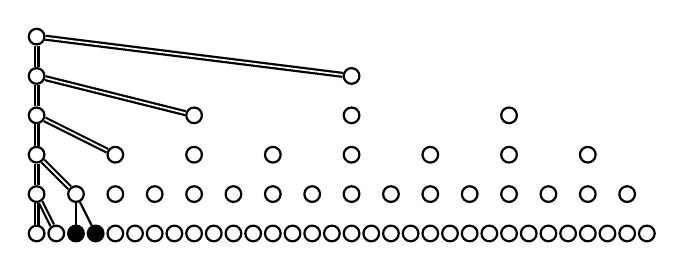
\begin{tikzpicture}[align=center]
      \node[draw=black, thick, fill=white, circle, inner sep=2pt] (T1) at (0,2.5) {};
      %
      \node[draw=black, thick, fill=white, circle, inner sep=2pt] (U2) at (0,2) {};
      \node[draw=black, thick, fill=white, circle, inner sep=2pt] (U3) at (4,2) {};
      %
      \node[draw=black, thick, fill=white, circle, inner sep=2pt] (V4) at (0,1.5) {};
      \node[draw=black, thick, fill=white, circle, inner sep=2pt] (V5) at (2,1.5) {};
      \node[draw=black, thick, circle, inner sep=2pt] (V6) at (4,1.5) {};
      \node[draw=black, thick, circle, inner sep=2pt] (V7) at (6,1.5) {};
      %
      \node[draw=black, thick, fill=white, circle, inner sep=2pt] (W8) at (0,1) {};
      \node[draw=black, thick, fill=white, circle, inner sep=2pt] (W9) at (1,1) {};
      \node[draw=black, thick, circle, inner sep=2pt] (W10) at (2,1) {};
      \node[draw=black, thick, circle, inner sep=2pt] (W11) at (3,1) {};
      \node[draw=black, thick, circle, inner sep=2pt] (W12) at (4,1) {};
      \node[draw=black, thick, circle, inner sep=2pt] (W13) at (5,1) {};
      \node[draw=black, thick, circle, inner sep=2pt] (W14) at (6,1) {};
      \node[draw=black, thick, circle, inner sep=2pt] (W15) at (7,1) {};
      %
      \node[draw=black, thick, fill=white, circle, inner sep=2pt] (X16) at (0,0.5) {};
      \node[draw=black, thick, fill=white, circle, inner sep=2pt] (X17) at (0.5,0.5) {};
      \node[draw=black, thick, fill=white, circle, inner sep=2pt] (X18) at (1,0.5) {};
      \node[draw=black, thick, fill=white, circle, inner sep=2pt] (X19) at (1.5,0.5) {};
      \node[draw=black, thick, fill=white, circle, inner sep=2pt] (X20) at (2,0.5) {};
      \node[draw=black, thick, fill=white, circle, inner sep=2pt] (X21) at (2.5,0.5) {}; 
      \node[draw=black, thick, fill=white, circle, inner sep=2pt] (X22) at (3,0.5) {};
      \node[draw=black, thick, fill=white, circle, inner sep=2pt] (X23) at (3.5,0.5) {};
      \node[draw=black, thick, fill=white, circle, inner sep=2pt] (X24) at (4,0.5) {};
      \node[draw=black, thick, fill=white, circle, inner sep=2pt] (X25) at (4.5,0.5) {};
      \node[draw=black, thick, fill=white, circle, inner sep=2pt] (X26) at (5,0.5) {};
      \node[draw=black, thick, fill=white, circle, inner sep=2pt] (X27) at (5.5,0.5) {};
      \node[draw=black, thick, fill=white, circle, inner sep=2pt] (X28) at (6,0.5) {};
      \node[draw=black, thick, fill=white, circle, inner sep=2pt] (X29) at (6.5,0.5) {};
      \node[draw=black, thick, fill=white, circle, inner sep=2pt] (X30) at (7,0.5) {};
      \node[draw=black, thick, fill=white, circle, inner sep=2pt] (X31) at (7.5,0.5) {};
      %
      \node[draw=black, thick, fill=white, circle, inner sep=2pt] (Y32) at (0,0) {};
      \node[draw=black, thick, fill=white, circle, inner sep=2pt] (Y33) at (0.25,0) {};
      \node[draw=black, thick, fill=black, circle, inner sep=2pt] (Y34) at (0.5,0) {};
      \node[draw=black, thick, fill=black, circle, inner sep=2pt] (Y35) at (0.75,0) {};
      \node[draw=black, thick, fill=white, circle, inner sep=2pt] (Y36) at (1,0) {};
      \node[draw=black, thick, fill=white, circle, inner sep=2pt] (Y37) at (1.25,0) {};
      \node[draw=black, thick, fill=white, circle, inner sep=2pt] (Y38) at (1.5,0) {};
      \node[draw=black, thick, fill=white, circle, inner sep=2pt] (Y39) at (1.75,0) {};
      \node[draw=black, thick, fill=white, circle, inner sep=2pt] (Y40) at (2,0) {};
      \node[draw=black, thick, fill=white, circle, inner sep=2pt] (Y41) at (2.25,0) {};
      \node[draw=black, thick, fill=white, circle, inner sep=2pt] (Y42) at (2.5,0) {};
      \node[draw=black, thick, fill=white, circle, inner sep=2pt] (Y43) at (2.75,0) {};
      \node[draw=black, thick, fill=white, circle, inner sep=2pt] (Y44) at (3,0) {};
      \node[draw=black, thick, fill=white, circle, inner sep=2pt] (Y45) at (3.25,0) {};
      \node[draw=black, thick, fill=white, circle, inner sep=2pt] (Y46) at (3.5,0) {};
      \node[draw=black, thick, fill=white, circle, inner sep=2pt] (Y47) at (3.75,0) {};
      \node[draw=black, thick, fill=white, circle, inner sep=2pt] (Y48) at (4,0) {};
      \node[draw=black, thick, fill=white, circle, inner sep=2pt] (Y49) at (4.25,0) {};
      \node[draw=black, thick, fill=white, circle, inner sep=2pt] (Y50) at (4.5,0) {};
      \node[draw=black, thick, fill=white, circle, inner sep=2pt] (Y51) at (4.75,0) {};
      \node[draw=black, thick, fill=white, circle, inner sep=2pt] (Y52) at (5,0) {};
      \node[draw=black, thick, fill=white, circle, inner sep=2pt] (Y53) at (5.25,0) {};
      \node[draw=black, thick, fill=white, circle, inner sep=2pt] (Y54) at (5.5,0) {};
      \node[draw=black, thick, fill=white, circle, inner sep=2pt] (Y55) at (5.75,0) {};
      \node[draw=black, thick, fill=white, circle, inner sep=2pt] (Y56) at (6,0) {};
      \node[draw=black, thick, fill=white, circle, inner sep=2pt] (Y57) at (6.25,0) {};
      \node[draw=black, thick, fill=white, circle, inner sep=2pt] (Y58) at (6.5,0) {};
      \node[draw=black, thick, fill=white, circle, inner sep=2pt] (Y59) at (6.75,0) {};
      \node[draw=black, thick, fill=white, circle, inner sep=2pt] (Y60) at (7,0) {};
      \node[draw=black, thick, fill=white, circle, inner sep=2pt] (Y61) at (7.25,0) {};
      \node[draw=black, thick, fill=white, circle, inner sep=2pt] (Y62) at (7.5,0) {};
      \node[draw=black, thick, fill=white, circle, inner sep=2pt] (Y63) at (7.75,0) {};
      %
      \draw[thick, double] (T1) -- (U2);
      \draw[thick, double] (T1) -- (U3);
      %
      \draw[thick, double] (U2) -- (V4);
      \draw[thick, double] (U2) -- (V5);
      %
      \draw[thick, double] (V4) -- (W8);
      \draw[thick, double] (V4) -- (W9);
      %
      \draw[thick, double] (W8) -- (X16);
      \draw[thick, double] (W8) -- (X17);
      %
      \draw[thick, double] (X16) -- (Y32);
      \draw[thick, double] (X16) -- (Y33);
      \draw[thick] (X17) -- (Y34);
      \draw[thick] (X17) -- (Y35);
      %
    \end{tikzpicture}
  \end{subfigure}
  \begin{subfigure}{\textwidth}
    \vspace{0.25cm}
    \centering
    \begin{tikzpicture}[align=center]
      \node[draw=black, line width=1.5pt, fill=black, cross out, inner sep=2pt] (T1) at (0,15.5) {};
      \node[draw=black, thick, fill=black, rectangle, inner sep=2.25pt] (T1) at (0.25,15.5) {};
      \node[draw=black, thick, fill=black, circle, inner sep=1.75pt] (T1) at (0.5,15.5) {};
      \node[draw=black, thick, fill=black, circle, inner sep=1.75pt] (T1) at (0.75,15.5) {};
      %
      \node[draw=white, thick, fill=white, circle, inner sep=2pt] (T1) at (7.75,15.5) {};
    \end{tikzpicture}
    % \caption{First packet: proof for leaf 0.}
  \end{subfigure}
  \begin{subfigure}{\textwidth}
    \vspace{0.25cm}
    \centering
    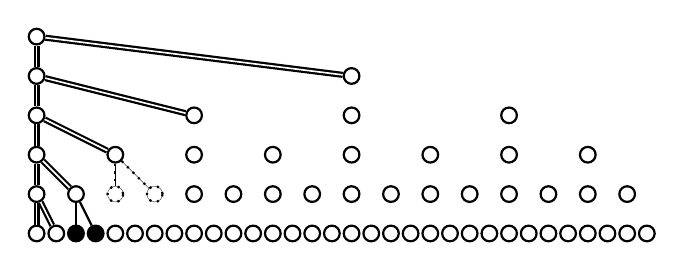
\begin{tikzpicture}[align=center]
      \node[draw=black, thick, fill=white, circle, inner sep=2pt] (T1) at (0,2.5) {};
      %
      \node[draw=black, thick, fill=white, circle, inner sep=2pt] (U2) at (0,2) {};
      \node[draw=black, thick, fill=white, circle, inner sep=2pt] (U3) at (4,2) {};
      %
      \node[draw=black, thick, fill=white, circle, inner sep=2pt] (V4) at (0,1.5) {};
      \node[draw=black, thick, fill=white, circle, inner sep=2pt] (V5) at (2,1.5) {};
      \node[draw=black, thick, fill=white, circle, inner sep=2pt] (V6) at (4,1.5) {};
      \node[draw=black, thick, fill=white, circle, inner sep=2pt] (V7) at (6,1.5) {};
      %
      \node[draw=black, thick, fill=white, circle, inner sep=2pt] (W8) at (0,1) {};
      \node[draw=black, thick, fill=white, circle, inner sep=2pt] (W9) at (1,1) {};
      \node[draw=black, thick, fill=white, circle, inner sep=2pt] (W10) at (2,1) {};
      \node[draw=black, thick, fill=white, circle, inner sep=2pt] (W11) at (3,1) {};
      \node[draw=black, thick, fill=white, circle, inner sep=2pt] (W12) at (4,1) {};
      \node[draw=black, thick, fill=white, circle, inner sep=2pt] (W13) at (5,1) {};
      \node[draw=black, thick, fill=white, circle, inner sep=2pt] (W14) at (6,1) {};
      \node[draw=black, thick, fill=white, circle, inner sep=2pt] (W15) at (7,1) {};
      %
      \node[draw=black, thick, fill=white, circle, inner sep=2pt] (X16) at (0,0.5) {};
      \node[draw=black, thick, fill=white, circle, inner sep=2pt] (X17) at (0.5,0.5) {};
      \node[draw=black, thick, dotted, fill=white, circle, inner sep=2pt] (X18) at (1,0.5) {};
      \node[draw=black, ultra thin, circle, inner sep=2pt] (X18) at (1,0.5) {};
      \node[draw=black, thick, dotted, fill=white, circle, inner sep=2pt] (X19) at (1.5,0.5) {};
      \node[draw=black, ultra thin, circle, inner sep=2pt] (X19) at (1.5,0.5) {};
      \node[draw=black, thick, fill=white, circle, inner sep=2pt] (X20) at (2,0.5) {};
      \node[draw=black, thick, fill=white, circle, inner sep=2pt] (X21) at (2.5,0.5) {}; 
      \node[draw=black, thick, fill=white, circle, inner sep=2pt] (X22) at (3,0.5) {};
      \node[draw=black, thick, fill=white, circle, inner sep=2pt] (X23) at (3.5,0.5) {};
      \node[draw=black, thick, fill=white, circle, inner sep=2pt] (X24) at (4,0.5) {};
      \node[draw=black, thick, fill=white, circle, inner sep=2pt] (X25) at (4.5,0.5) {};
      \node[draw=black, thick, fill=white, circle, inner sep=2pt] (X26) at (5,0.5) {};
      \node[draw=black, thick, fill=white, circle, inner sep=2pt] (X27) at (5.5,0.5) {};
      \node[draw=black, thick, fill=white, circle, inner sep=2pt] (X28) at (6,0.5) {};
      \node[draw=black, thick, fill=white, circle, inner sep=2pt] (X29) at (6.5,0.5) {};
      \node[draw=black, thick, fill=white, circle, inner sep=2pt] (X30) at (7,0.5) {};
      \node[draw=black, thick, fill=white, circle, inner sep=2pt] (X31) at (7.5,0.5) {};
      %
      \node[draw=black, thick, fill=white, circle, inner sep=2pt] (Y32) at (0,0) {};
      \node[draw=black, thick, fill=white, circle, inner sep=2pt] (Y33) at (0.25,0) {};
      \node[draw=black, thick, fill=black, circle, inner sep=2pt] (Y34) at (0.5,0) {};
      \node[draw=black, thick, fill=black, circle, inner sep=2pt] (Y35) at (0.75,0) {};
      \node[draw=black, thick, circle, fill=white, inner sep=2pt] (Y36) at (1,0) {};
      \node[draw=black, thick, circle, fill=white, inner sep=2pt] (Y37) at (1.25,0) {};
      \node[draw=black, thick, fill=white, circle, inner sep=2pt] (Y38) at (1.5,0) {};
      \node[draw=black, thick, fill=white, circle, inner sep=2pt] (Y39) at (1.75,0) {};
      \node[draw=black, thick, fill=white, circle, inner sep=2pt] (Y40) at (2,0) {};
      \node[draw=black, thick, fill=white, circle, inner sep=2pt] (Y41) at (2.25,0) {};
      \node[draw=black, thick, fill=white, circle, inner sep=2pt] (Y42) at (2.5,0) {};
      \node[draw=black, thick, fill=white, circle, inner sep=2pt] (Y43) at (2.75,0) {};
      \node[draw=black, thick, fill=white, circle, inner sep=2pt] (Y44) at (3,0) {};
      \node[draw=black, thick, fill=white, circle, inner sep=2pt] (Y45) at (3.25,0) {};
      \node[draw=black, thick, fill=white, circle, inner sep=2pt] (Y46) at (3.5,0) {};
      \node[draw=black, thick, fill=white, circle, inner sep=2pt] (Y47) at (3.75,0) {};
      \node[draw=black, thick, fill=white, circle, inner sep=2pt] (Y48) at (4,0) {};
      \node[draw=black, thick, fill=white, circle, inner sep=2pt] (Y49) at (4.25,0) {};
      \node[draw=black, thick, fill=white, circle, inner sep=2pt] (Y50) at (4.5,0) {};
      \node[draw=black, thick, fill=white, circle, inner sep=2pt] (Y51) at (4.75,0) {};
      \node[draw=black, thick, fill=white, circle, inner sep=2pt] (Y52) at (5,0) {};
      \node[draw=black, thick, fill=white, circle, inner sep=2pt] (Y53) at (5.25,0) {};
      \node[draw=black, thick, fill=white, circle, inner sep=2pt] (Y54) at (5.5,0) {};
      \node[draw=black, thick, fill=white, circle, inner sep=2pt] (Y55) at (5.75,0) {};
      \node[draw=black, thick, fill=white, circle, inner sep=2pt] (Y56) at (6,0) {};
      \node[draw=black, thick, fill=white, circle, inner sep=2pt] (Y57) at (6.25,0) {};
      \node[draw=black, thick, fill=white, circle, inner sep=2pt] (Y58) at (6.5,0) {};
      \node[draw=black, thick, fill=white, circle, inner sep=2pt] (Y59) at (6.75,0) {};
      \node[draw=black, thick, fill=white, circle, inner sep=2pt] (Y60) at (7,0) {};
      \node[draw=black, thick, fill=white, circle, inner sep=2pt] (Y61) at (7.25,0) {};
      \node[draw=black, thick, fill=white, circle, inner sep=2pt] (Y62) at (7.5,0) {};
      \node[draw=black, thick, fill=white, circle, inner sep=2pt] (Y63) at (7.75,0) {};
      %
      \draw[thick, double] (T1) -- (U2);
      \draw[thick, double] (T1) -- (U3);
      %
      \draw[thick, double] (U2) -- (V4);
      \draw[thick, double] (U2) -- (V5);
      %
      \draw[thick, double] (V4) -- (W8);
      \draw[thick, double] (V4) -- (W9);
      %
      \draw[thick, double] (W8) -- (X16);
      \draw[thick, double] (W8) -- (X17);
      \draw[thick, dotted] (W9) -- (X18);
      \draw[ultra thin] (W9) -- (X18);
      \draw[thick, dotted] (W9) -- (X19);
      \draw[ultra thin] (W9) -- (X19);
      %
      \draw[thick, double] (X16) -- (Y32);
      \draw[thick, double] (X16) -- (Y33);
      \draw[thick] (X17) -- (Y34);
      \draw[thick] (X17) -- (Y35);
    \end{tikzpicture}
  \end{subfigure}
  \begin{subfigure}{\textwidth}
    \vspace{0.25cm}
    \centering
    \begin{tikzpicture}[align=center]
      \node[draw=black, line width=1.5pt, fill=black, cross out, inner sep=2pt] (T1) at (0,15.5) {};
      \node[draw=black, thick, fill=black, rectangle, inner sep=2.25pt] (T1) at (0.25,15.5) {};
      \node[draw=black, thick, fill=black, circle, inner sep=1.75pt] (T1) at (0.5,15.5) {};
      \node[draw=black, thick, fill=black, circle, inner sep=1.75pt] (T1) at (0.75,15.5) {};
      %
      \node[draw=black, thick, dotted, fill=white, rectangle, inner sep=2.25pt] (T1) at (0.5,15.25) {};
      \node[draw=black, ultra thin, rectangle, inner sep=2.25pt] (T1) at (0.5,15.25) {};
      \node[draw=black, thick, dotted, fill=white, circle, inner sep=1.75pt] (T1) at (1.0,15.25) {};
      \node[draw=black, ultra thin, circle, inner sep=1.75pt] (T1) at (1.0,15.25) {};
      \node[draw=black, thick, dotted, fill=white, circle, inner sep=1.75pt] (T1) at (1.5,15.25) {};
      \node[draw=black, ultra thin, circle, inner sep=1.75pt] (T1) at (1.5,15.25) {};
      %
      \node[draw=white, thick, fill=white, circle, inner sep=2pt] (T1) at (7.75,15.5) {};
    \end{tikzpicture}
    % \caption{Second packet: proof for leaf 1.}
  \end{subfigure}
  \begin{subfigure}{\textwidth}
    \vspace{0.25cm}
    \centering
    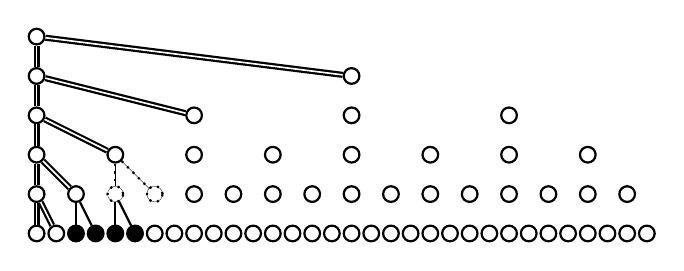
\begin{tikzpicture}[align=center]
      \node[draw=black, thick, fill=white, circle, inner sep=2pt] (T1) at (0,2.5) {};
      %
      \node[draw=black, thick, fill=white, circle, inner sep=2pt] (U2) at (0,2) {};
      \node[draw=black, thick, fill=white, circle, inner sep=2pt] (U3) at (4,2) {};
      %
      \node[draw=black, thick, fill=white, circle, inner sep=2pt] (V4) at (0,1.5) {};
      \node[draw=black, thick, fill=white, circle, inner sep=2pt] (V5) at (2,1.5) {};
      \node[draw=black, thick, fill=white, circle, inner sep=2pt] (V6) at (4,1.5) {};
      \node[draw=black, thick, fill=white, circle, inner sep=2pt] (V7) at (6,1.5) {};
      %
      \node[draw=black, thick, fill=white, circle, inner sep=2pt] (W8) at (0,1) {};
      \node[draw=black, thick, fill=white, circle, inner sep=2pt] (W9) at (1,1) {};
      \node[draw=black, thick, fill=white, circle, inner sep=2pt] (W10) at (2,1) {};
      \node[draw=black, thick, fill=white, circle, inner sep=2pt] (W11) at (3,1) {};
      \node[draw=black, thick, fill=white, circle, inner sep=2pt] (W12) at (4,1) {};
      \node[draw=black, thick, fill=white, circle, inner sep=2pt] (W13) at (5,1) {};
      \node[draw=black, thick, fill=white, circle, inner sep=2pt] (W14) at (6,1) {};
      \node[draw=black, thick, fill=white, circle, inner sep=2pt] (W15) at (7,1) {};
      %
      \node[draw=black, thick, fill=white, circle, inner sep=2pt] (X16) at (0,0.5) {};
      \node[draw=black, thick, fill=white, circle, inner sep=2pt] (X17) at (0.5,0.5) {};
      \node[draw=black, thick, dotted, fill=white, circle, inner sep=2pt] (X18) at (1,0.5) {};
      \node[draw=black, ultra thin, circle, inner sep=2pt] (X18) at (1,0.5) {};
      \node[draw=black, thick, dotted, fill=white, circle, inner sep=2pt] (X19) at (1.5,0.5) {};
      \node[draw=black, ultra thin, circle, inner sep=2pt] (X19) at (1.5,0.5) {};
      \node[draw=black, thick, fill=white, circle, inner sep=2pt] (X20) at (2,0.5) {};
      \node[draw=black, thick, fill=white, circle, inner sep=2pt] (X21) at (2.5,0.5) {}; 
      \node[draw=black, thick, fill=white, circle, inner sep=2pt] (X22) at (3,0.5) {};
      \node[draw=black, thick, fill=white, circle, inner sep=2pt] (X23) at (3.5,0.5) {};
      \node[draw=black, thick, fill=white, circle, inner sep=2pt] (X24) at (4,0.5) {};
      \node[draw=black, thick, fill=white, circle, inner sep=2pt] (X25) at (4.5,0.5) {};
      \node[draw=black, thick, fill=white, circle, inner sep=2pt] (X26) at (5,0.5) {};
      \node[draw=black, thick, fill=white, circle, inner sep=2pt] (X27) at (5.5,0.5) {};
      \node[draw=black, thick, fill=white, circle, inner sep=2pt] (X28) at (6,0.5) {};
      \node[draw=black, thick, fill=white, circle, inner sep=2pt] (X29) at (6.5,0.5) {};
      \node[draw=black, thick, fill=white, circle, inner sep=2pt] (X30) at (7,0.5) {};
      \node[draw=black, thick, fill=white, circle, inner sep=2pt] (X31) at (7.5,0.5) {};
      %
      \node[draw=black, thick, fill=white, circle, inner sep=2pt] (Y32) at (0,0) {};
      \node[draw=black, thick, fill=white, circle, inner sep=2pt] (Y33) at (0.25,0) {};
      \node[draw=black, thick, fill=black, circle, inner sep=2pt] (Y34) at (0.5,0) {};
      \node[draw=black, thick, fill=black, circle, inner sep=2pt] (Y35) at (0.75,0) {};
      \node[draw=black, thick, circle, fill=black, inner sep=2pt] (Y36) at (1,0) {};
      \node[draw=black, thick, circle, fill=black, inner sep=2pt] (Y37) at (1.25,0) {};
      \node[draw=black, thick, fill=white, circle, inner sep=2pt] (Y38) at (1.5,0) {};
      \node[draw=black, thick, fill=white, circle, inner sep=2pt] (Y39) at (1.75,0) {};
      \node[draw=black, thick, fill=white, circle, inner sep=2pt] (Y40) at (2,0) {};
      \node[draw=black, thick, fill=white, circle, inner sep=2pt] (Y41) at (2.25,0) {};
      \node[draw=black, thick, fill=white, circle, inner sep=2pt] (Y42) at (2.5,0) {};
      \node[draw=black, thick, fill=white, circle, inner sep=2pt] (Y43) at (2.75,0) {};
      \node[draw=black, thick, fill=white, circle, inner sep=2pt] (Y44) at (3,0) {};
      \node[draw=black, thick, fill=white, circle, inner sep=2pt] (Y45) at (3.25,0) {};
      \node[draw=black, thick, fill=white, circle, inner sep=2pt] (Y46) at (3.5,0) {};
      \node[draw=black, thick, fill=white, circle, inner sep=2pt] (Y47) at (3.75,0) {};
      \node[draw=black, thick, fill=white, circle, inner sep=2pt] (Y48) at (4,0) {};
      \node[draw=black, thick, fill=white, circle, inner sep=2pt] (Y49) at (4.25,0) {};
      \node[draw=black, thick, fill=white, circle, inner sep=2pt] (Y50) at (4.5,0) {};
      \node[draw=black, thick, fill=white, circle, inner sep=2pt] (Y51) at (4.75,0) {};
      \node[draw=black, thick, fill=white, circle, inner sep=2pt] (Y52) at (5,0) {};
      \node[draw=black, thick, fill=white, circle, inner sep=2pt] (Y53) at (5.25,0) {};
      \node[draw=black, thick, fill=white, circle, inner sep=2pt] (Y54) at (5.5,0) {};
      \node[draw=black, thick, fill=white, circle, inner sep=2pt] (Y55) at (5.75,0) {};
      \node[draw=black, thick, fill=white, circle, inner sep=2pt] (Y56) at (6,0) {};
      \node[draw=black, thick, fill=white, circle, inner sep=2pt] (Y57) at (6.25,0) {};
      \node[draw=black, thick, fill=white, circle, inner sep=2pt] (Y58) at (6.5,0) {};
      \node[draw=black, thick, fill=white, circle, inner sep=2pt] (Y59) at (6.75,0) {};
      \node[draw=black, thick, fill=white, circle, inner sep=2pt] (Y60) at (7,0) {};
      \node[draw=black, thick, fill=white, circle, inner sep=2pt] (Y61) at (7.25,0) {};
      \node[draw=black, thick, fill=white, circle, inner sep=2pt] (Y62) at (7.5,0) {};
      \node[draw=black, thick, fill=white, circle, inner sep=2pt] (Y63) at (7.75,0) {};
      %
      \draw[thick, double] (T1) -- (U2);
      \draw[thick, double] (T1) -- (U3);
      %
      \draw[thick, double] (U2) -- (V4);
      \draw[thick, double] (U2) -- (V5);
      %
      \draw[thick, double] (V4) -- (W8);
      \draw[thick, double] (V4) -- (W9);
      %
      \draw[thick, double] (W8) -- (X16);
      \draw[thick, double] (W8) -- (X17);
      \draw[thick, dotted] (W9) -- (X18);
      \draw[ultra thin] (W9) -- (X18);
      \draw[thick, dotted] (W9) -- (X19);
      \draw[ultra thin] (W9) -- (X19);
      %
      \draw[thick, double] (X16) -- (Y32);
      \draw[thick, double] (X16) -- (Y33);
      \draw[thick] (X17) -- (Y34);
      \draw[thick] (X17) -- (Y35);
      \draw[thick] (X18) -- (Y36);
      \draw[thick] (X18) -- (Y37);
    \end{tikzpicture}
  \end{subfigure}
  \begin{subfigure}{\textwidth}
    \vspace{0.25cm}
    \centering
    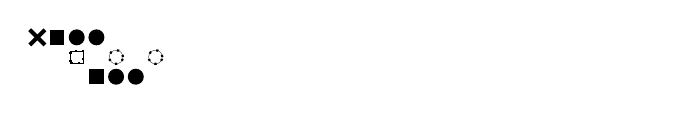
\begin{tikzpicture}[align=center]
      \node[draw=black, line width=1.5pt, fill=black, cross out, inner sep=2pt] (T1) at (0,15.5) {};
      \node[draw=black, thick, fill=black, rectangle, inner sep=2.25pt] (T1) at (0.25,15.5) {};
      \node[draw=black, thick, fill=black, circle, inner sep=1.75pt] (T1) at (0.5,15.5) {};
      \node[draw=black, thick, fill=black, circle, inner sep=1.75pt] (T1) at (0.75,15.5) {};
      %
      \node[draw=black, thick, dotted, fill=white, rectangle, inner sep=2.25pt] (T1) at (0.5,15.25) {};
      \node[draw=black, ultra thin, rectangle, inner sep=2.25pt] (T1) at (0.5,15.25) {};
      \node[draw=black, thick, dotted, fill=white, circle, inner sep=1.75pt] (T1) at (1.0,15.25) {};
      \node[draw=black, ultra thin, circle, inner sep=1.75pt] (T1) at (1.0,15.25) {};
      \node[draw=black, thick, dotted, fill=white, circle, inner sep=1.75pt] (T1) at (1.5,15.25) {};
      \node[draw=black, ultra thin, circle, inner sep=1.75pt] (T1) at (1.5,15.25) {};
      %
      \node[draw=black, thick, fill=black, rectangle, inner sep=2.25pt] (T1) at (0.75,15.0) {};
      \node[draw=black, thick, fill=black, circle, inner sep=1.75pt] (T1) at (1,15.0) {};
      \node[draw=black, thick, fill=black, circle, inner sep=1.75pt] (T1) at (1.25,15.0) {};
      %
      \node[draw=white, thick, fill=white, circle, inner sep=2pt] (T1) at (7.75,15.5) {};
    \end{tikzpicture}
    % \caption{Third packet: proof for leaf 2.}
  \end{subfigure}
  \begin{subfigure}{\textwidth}
    \vspace{0.25cm}
    \centering
    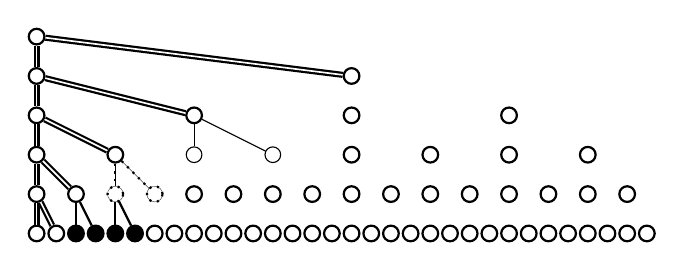
\begin{tikzpicture}[align=center]
      \node[draw=black, thick, fill=white, circle, inner sep=2pt] (T1) at (0,2.5) {};
      %
      \node[draw=black, thick, fill=white, circle, inner sep=2pt] (U2) at (0,2) {};
      \node[draw=black, thick, fill=white, circle, inner sep=2pt] (U3) at (4,2) {};
      %
      \node[draw=black, thick, fill=white, circle, inner sep=2pt] (V4) at (0,1.5) {};
      \node[draw=black, thick, fill=white, circle, inner sep=2pt] (V5) at (2,1.5) {};
      \node[draw=black, thick, fill=white, circle, inner sep=2pt] (V6) at (4,1.5) {};
      \node[draw=black, thick, fill=white, circle, inner sep=2pt] (V7) at (6,1.5) {};
      %
      \node[draw=black, thick, fill=white, circle, inner sep=2pt] (W8) at (0,1) {};
      \node[draw=black, thick, fill=white, circle, inner sep=2pt] (W9) at (1,1) {};
      \node[draw=black, fill=white, circle, inner sep=2pt] (W10) at (2,1) {};
      \node[draw=black, fill=white, circle, inner sep=2pt] (W11) at (3,1) {};
      \node[draw=black, thick, fill=white, circle, inner sep=2pt] (W12) at (4,1) {};
      \node[draw=black, thick, fill=white, circle, inner sep=2pt] (W13) at (5,1) {};
      \node[draw=black, thick, fill=white, circle, inner sep=2pt] (W14) at (6,1) {};
      \node[draw=black, thick, fill=white, circle, inner sep=2pt] (W15) at (7,1) {};
      %
      \node[draw=black, thick, fill=white, circle, inner sep=2pt] (X16) at (0,0.5) {};
      \node[draw=black, thick, fill=white, circle, inner sep=2pt] (X17) at (0.5,0.5) {};
      \node[draw=black, thick, dotted, fill=white, circle, inner sep=2pt] (X18) at (1,0.5) {};
      \node[draw=black, ultra thin, circle, inner sep=2pt] (X18) at (1,0.5) {};
      \node[draw=black, thick, dotted, fill=white, circle, inner sep=2pt] (X19) at (1.5,0.5) {};
      \node[draw=black, ultra thin, circle, inner sep=2pt] (X19) at (1.5,0.5) {};
      \node[draw=black, thick, fill=white, circle, inner sep=2pt] (X20) at (2,0.5) {};
      \node[draw=black, thick, fill=white, circle, inner sep=2pt] (X21) at (2.5,0.5) {}; 
      \node[draw=black, thick, fill=white, circle, inner sep=2pt] (X22) at (3,0.5) {};
      \node[draw=black, thick, fill=white, circle, inner sep=2pt] (X23) at (3.5,0.5) {};
      \node[draw=black, thick, fill=white, circle, inner sep=2pt] (X24) at (4,0.5) {};
      \node[draw=black, thick, fill=white, circle, inner sep=2pt] (X25) at (4.5,0.5) {};
      \node[draw=black, thick, fill=white, circle, inner sep=2pt] (X26) at (5,0.5) {};
      \node[draw=black, thick, fill=white, circle, inner sep=2pt] (X27) at (5.5,0.5) {};
      \node[draw=black, thick, fill=white, circle, inner sep=2pt] (X28) at (6,0.5) {};
      \node[draw=black, thick, fill=white, circle, inner sep=2pt] (X29) at (6.5,0.5) {};
      \node[draw=black, thick, fill=white, circle, inner sep=2pt] (X30) at (7,0.5) {};
      \node[draw=black, thick, fill=white, circle, inner sep=2pt] (X31) at (7.5,0.5) {};
      %
      \node[draw=black, thick, fill=white, circle, inner sep=2pt] (Y32) at (0,0) {};
      \node[draw=black, thick, fill=white, circle, inner sep=2pt] (Y33) at (0.25,0) {};
      \node[draw=black, thick, fill=black, circle, inner sep=2pt] (Y34) at (0.5,0) {};
      \node[draw=black, thick, fill=black, circle, inner sep=2pt] (Y35) at (0.75,0) {};
      \node[draw=black, thick, circle, fill=black, inner sep=2pt] (Y36) at (1,0) {};
      \node[draw=black, thick, circle, fill=black, inner sep=2pt] (Y37) at (1.25,0) {};
      \node[draw=black, thick, fill=white, circle, inner sep=2pt] (Y38) at (1.5,0) {};
      \node[draw=black, thick, fill=white, circle, inner sep=2pt] (Y39) at (1.75,0) {};
      \node[draw=black, thick, fill=white, circle, inner sep=2pt] (Y40) at (2,0) {};
      \node[draw=black, thick, fill=white, circle, inner sep=2pt] (Y41) at (2.25,0) {};
      \node[draw=black, thick, fill=white, circle, inner sep=2pt] (Y42) at (2.5,0) {};
      \node[draw=black, thick, fill=white, circle, inner sep=2pt] (Y43) at (2.75,0) {};
      \node[draw=black, thick, fill=white, circle, inner sep=2pt] (Y44) at (3,0) {};
      \node[draw=black, thick, fill=white, circle, inner sep=2pt] (Y45) at (3.25,0) {};
      \node[draw=black, thick, fill=white, circle, inner sep=2pt] (Y46) at (3.5,0) {};
      \node[draw=black, thick, fill=white, circle, inner sep=2pt] (Y47) at (3.75,0) {};
      \node[draw=black, thick, fill=white, circle, inner sep=2pt] (Y48) at (4,0) {};
      \node[draw=black, thick, fill=white, circle, inner sep=2pt] (Y49) at (4.25,0) {};
      \node[draw=black, thick, fill=white, circle, inner sep=2pt] (Y50) at (4.5,0) {};
      \node[draw=black, thick, fill=white, circle, inner sep=2pt] (Y51) at (4.75,0) {};
      \node[draw=black, thick, fill=white, circle, inner sep=2pt] (Y52) at (5,0) {};
      \node[draw=black, thick, fill=white, circle, inner sep=2pt] (Y53) at (5.25,0) {};
      \node[draw=black, thick, fill=white, circle, inner sep=2pt] (Y54) at (5.5,0) {};
      \node[draw=black, thick, fill=white, circle, inner sep=2pt] (Y55) at (5.75,0) {};
      \node[draw=black, thick, fill=white, circle, inner sep=2pt] (Y56) at (6,0) {};
      \node[draw=black, thick, fill=white, circle, inner sep=2pt] (Y57) at (6.25,0) {};
      \node[draw=black, thick, fill=white, circle, inner sep=2pt] (Y58) at (6.5,0) {};
      \node[draw=black, thick, fill=white, circle, inner sep=2pt] (Y59) at (6.75,0) {};
      \node[draw=black, thick, fill=white, circle, inner sep=2pt] (Y60) at (7,0) {};
      \node[draw=black, thick, fill=white, circle, inner sep=2pt] (Y61) at (7.25,0) {};
      \node[draw=black, thick, fill=white, circle, inner sep=2pt] (Y62) at (7.5,0) {};
      \node[draw=black, thick, fill=white, circle, inner sep=2pt] (Y63) at (7.75,0) {};
      %
      \draw[thick, double] (T1) -- (U2);
      \draw[thick, double] (T1) -- (U3);
      %
      \draw[thick, double] (U2) -- (V4);
      \draw[thick, double] (U2) -- (V5);
      %
      \draw[thick, double] (V4) -- (W8);
      \draw[thick, double] (V4) -- (W9);
      \draw[] (V5) -- (W10);
      \draw[] (V5) -- (W11);
      %
      \draw[thick, double] (W8) -- (X16);
      \draw[thick, double] (W8) -- (X17);
      \draw[thick, dotted] (W9) -- (X18);
      \draw[ultra thin] (W9) -- (X18);
      \draw[thick, dotted] (W9) -- (X19);
      \draw[ultra thin] (W9) -- (X19);
      %
      \draw[thick, double] (X16) -- (Y32);
      \draw[thick, double] (X16) -- (Y33);
      \draw[thick] (X17) -- (Y34);
      \draw[thick] (X17) -- (Y35);
      \draw[thick] (X18) -- (Y36);
      \draw[thick] (X18) -- (Y37);
    \end{tikzpicture}
  \end{subfigure}
  \begin{subfigure}{\textwidth}
    \vspace{0.25cm}
    \centering
    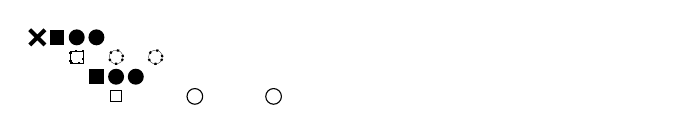
\begin{tikzpicture}[align=center]
      \node[draw=black, line width=1.5pt, fill=black, cross out, inner sep=2pt] (T1) at (0,15.5) {};
      \node[draw=black, thick, fill=black, rectangle, inner sep=2.25pt] (T1) at (0.25,15.5) {};
      \node[draw=black, thick, fill=black, circle, inner sep=1.75pt] (T1) at (0.5,15.5) {};
      \node[draw=black, thick, fill=black, circle, inner sep=1.75pt] (T1) at (0.75,15.5) {};
      %
      \node[draw=black, thick, dotted, fill=white, rectangle, inner sep=2.25pt] (T1) at (0.5,15.25) {};
      \node[draw=black, ultra thin, rectangle, inner sep=2.25pt] (T1) at (0.5,15.25) {};
      \node[draw=black, thick, dotted, fill=white, circle, inner sep=1.75pt] (T1) at (1.0,15.25) {};
      \node[draw=black, ultra thin, circle, inner sep=1.75pt] (T1) at (1.0,15.25) {};
      \node[draw=black, thick, dotted, fill=white, circle, inner sep=1.75pt] (T1) at (1.5,15.25) {};
      \node[draw=black, ultra thin, circle, inner sep=1.75pt] (T1) at (1.5,15.25) {};
      %
      \node[draw=black, thick, fill=black, rectangle, inner sep=2.25pt] (T1) at (0.75,15.0) {};
      \node[draw=black, thick, fill=black, circle, inner sep=1.75pt] (T1) at (1,15.0) {};
      \node[draw=black, thick, fill=black, circle, inner sep=1.75pt] (T1) at (1.25,15.0) {};
      %
      \node[draw=black, fill=white, rectangle, inner sep=2pt] (T1) at (1,14.75) {};
      \node[draw=black, fill=white, circle, inner sep=2pt] (T1) at (2,14.75) {};
      \node[draw=black, fill=white, circle, inner sep=2pt] (T1) at (3,14.75) {};
      %
      \node[draw=white, thick, fill=white, circle, inner sep=2pt] (T1) at (7.75,15.5) {};
    \end{tikzpicture}
    % \caption{Fourth packet: proof for leaf 3.}
  \end{subfigure}
  \caption{Lackman-ordered traversal as time series.}
  \label{fig:lackman-2}
\end{figure}


Compared to Blackman ordering, the pairs appear offset by one position, which simplifies the bit-manipulation logic for computing which pair to include in each packet.

There's one more optimization worth mentioning: If the message is small enough, we can skip the initial step of sending a packet containing only a Merkle proof (with no leaf data). Obviously, for a one-leaf message, we can simply send that leaf; the hash of that leaf is the Merkle root. For a two-leaf message, we can send the leaf plus its sibling hash (\lstinline[style=inlinecode]{[1,2)}); the verifier can hash the first leaf and combine it with the sibling hash to recover the root. And for a three- or four-leaf message, we can send \lstinline[style=inlinecode]{[1,2)} and \lstinline[style=inlinecode]{[2,3)} (or \lstinline[style=inlinecode]{[2,4)}, respectively). That's the limit, though; if a message has five leaves, we would need to send at least three sibling hashes for the verifier to recompute the root, but our packet framing only allows up to two hashes.

\subsubsection{Arena Allocator}
\label{arena-allocator}

Directed Messaging uses a simple bump allocator arena for memory
management. Each arena is a contiguous block of memory with three
pointers: the start of the allocation (\texttt{dat}), the current
allocation position (\texttt{beg}), and the end of the block
(\texttt{end}). The \texttt{new()} macro allocates objects by advancing
the \texttt{beg} pointer with proper alignment.

The arena allocator provides \emph{no individual deallocation} -- once memory is allocated from an arena, it can't be freed separately. Instead, the entire arena is freed at once when the data structure that owns it is destroyed.

\paragraph{Allocation Patterns}
\label{allocation-patterns}

Arenas are created with sizes tailored to their use case:

\begin{itemize}
  \item  \textbf{Pending Interest Table entries} use 16~KiB arenas.  These store lane addresses for pending requests, with the arena holding  the entry itself plus a linked list of address records.
  \item  \textbf{Pending requests} allocate arenas at 5× the expected message size. A request receiving a 1~MiB message gets a 5~MiB arena.  This single arena holds the request state, fragment data buffer, \textsc{lss} authentication pairs, packet statistics, bitset tracking received fragments, and pre-serialized request packets.
  \item  \textbf{Jumbo frame cache entries} allocate based on proof size, data size, hash pairs, plus a 2~KiB buffer. For a 1~MiB message, this might be around 1--2~MiB. The arena stores the cached response data, Merkle proof spine, and authentication hashes.
  \item  \textbf{Temporary arenas} for packet sending use message size plus 16~KiB to hold serialized packets plus overhead.
  \item  \textbf{Scry callbacks} get small arenas for asynchronous Arvo interactions.
\end{itemize}

\paragraph{Deallocation Triggers}\label{deallocation-triggers}

Arenas are freed only when their parent data structure is destroyed:

\begin{itemize}
  \item  \textbf{Request completion}: When all fragments arrive, the request is deleted and its arena freed. This happens asynchronously through \texttt{libuv}'s handle cleanup to ensure proper timer shutdown before freeing memory.
  \item  \textbf{Authentication failure}: If \textsc{lss} verification fails while processing fragments, the entire request is immediately deleted.
  \item  \textbf{Timeout expiration}: When retry timers exhaust their attempts, the request is deleted.
  \item  \textbf{\textsc{pit} expiration}: After 20 seconds, entries are cleaned from the Pending Interest Table.
  \item  \textbf{Cache eviction}: When the jumbo cache exceeds 200~MiB, it's entirely cleared and all cached arenas are freed.
\end{itemize}

\paragraph{Lifecycle}\label{lifecycle}

A typical request lifecycle:

\begin{enumerate}
  \item  \textbf{Allocation}: Receive initial packet, create arena with 5× data size, allocate all request state from arena.
  \item  \textbf{Growth}: As fragments arrive, write into pre-allocated buffers within the arena.
  \item  \textbf{Completion}: All fragments received, construct final message, send to Arvo.
  \item  \textbf{Cleanup}: Delete request from map, stop timer, close handle asynchronously.
  \item  \textbf{Deallocation}: In UV callback, free entire arena with single call.
\end{enumerate}

This design trades memory efficiency for speed. Arenas may hold unused space, but allocation is extremely fast (just pointer arithmetic), and the single-free design eliminates per-object deallocation overhead and fragmentation issues.

\subsubsection{Download Checkpointing}\label{download-checkpointing}

This has not been deployed to the network, but this design allows the requesting ship's runtime to inject jumbo frames of arbitrary size into its Arvo as each one finishes downloading, with real authentication by using Lockstep. Arvo will seamlessly store those jumbo frames and accumulate them until it has the whole message, at which time it will deserialize the message into an Urbit `noun' data structure and deliver it to the application or kernel module that had triggered the request.

This allows the system to make effective use of Arvo as a download checkpointing system. After a process crash, machine restart, or any other transient failure, the download can be resumed with minimal loss of information.

Injecting an authenticated jumbo frame into Arvo maintains a security boundary. Urbit's main runtime, Vere, has two Unix processes: one runs the Arvo kernel, and the other handles input and output. Arvo maintains ultimate responsibility for cryptographic operations. This lets the private key remain solely in the Arvo process, leaving the I/O process without the ability to encrypt, decrypt, authenticate, or verify authentication.

Instead, the runtime delegates any operation requiring a private key to Arvo, including validating the message-level authentication in the first packet of a scry response. To add a layer of defense in depth in case the I/O process is compromised, Arvo performs its own packet validation, including the Lockstep packet authentication. This remains efficient because each packet can be a large jumbo frame.

Checkpointing has another benefit. No matter how large a message is, the downloader can keep a fixed upper bound on the memory footprint while download that message, proportional to one jumbo frame.

\subsubsection{Download Resumption}
\label{download-resumption}

After a transient failure -- most commonly a process crash or machine restart -- a requesting ship can resume a download. In order to pick up from where it left off, the runtime first asks its local Arvo for the leaf-packet hashes it needs, which Arvo generates on demand from the jumbo frames that have already been downloaded and stored in Arvo. This is $O(\log(n))$ hashes, where $n$ is the message length, and no message data needs to be sent over inter-process communication in order to resume a download, preventing restarts from becoming slow and memory-intensive.

Once the runtime has the hashes it needs, it resumes the Lockstep streaming verification that it had been doing, beginning with the next jumbo frame after the last one that had been downloaded and saved in Arvo.

Download checkpointing and resumption together provide a good set of tools for download management. This is beyond what \textsc{tcp} provides, or even \textsc{http}. \textsc{http} has resumption headers, but both client and server have to opt into using them, so in practice many \textsc{http}-based downloads cannot be resumed.

\section{Congestion Control}
\label{congestion-control}

In Directed Messaging, congestion control is pluggable. The requesting ship decides how many request packets to send and at what time. The publisher ship is only responsible for responding to requests and does not participate in congestion control.

It is possible for an Urbit implementation to have functioning, if not performant, networking, without any runtime implementation of congestion control. The formal specification in the networking module of the Arvo kernel for how a ship sends request packets is a simple one-at-a-time indefinite repeating timer. The ship sends the first request packet, repeating it every thirty seconds until a response packet is heard, at which point it begins requesting the next packet.

Performant congestion control, then, is an extension of Urbit's idea of a ``jet'', i.\,e.\ a peephole optimization that replaces a built-in function, defined formally but is likely slow, with an optimized low-level implementation.

In practice, this slow packet re-send is used for retrying dead connections, where the publishing ship has been unresponsive for a long time. This is important because Urbit network requests generally do not time out at the application level; they are considered persistent, and they must be retried indefinitely. Fast, runtime-based congestion control only kicks in when the runtime receives a response packet, indicating the publishing ship has become responsive.

The current implementation of Directed Messaging employs a modified \textsc{tcp} Tahoe-style congestion control algorithm adapted to its request/response architecture and packet-oriented nature. The protocol's congestion control differs from traditional \textsc{tcp} in several fundamental ways due to its pull-based communication model and implicit acknowledgment scheme.

\subsection{Architectural Foundation}
\label{architectural-foundation}

Unlike \textsc{tcp}'s push-based model where senders transmit data and await separate acknowledgment packets, Directed Messaging operates on a request/response paradigm. The requesting ship sends \textsc{peek} packets to solicit specific fragments, and the responding ship sends \textsc{page} packets containing the requested data. The arrival of each \textsc{page} packet serves as an implicit acknowledgment -- no separate \textsc{ack} packets exist in the protocol. This inversion places congestion control responsibility on the requester rather than the sender, allowing the party pulling data to directly regulate network load.

The protocol operates on fixed-size fragments rather than byte streams. Each fragment contains up to 1024 bytes of payload data (at the default \lstinline[style=inlinecode]{$bloq} parameter of 13). The congestion window (\lstinline[style=inlinecode]{cwnd}) measures capacity in fragment count rather than bytes, providing coarser but simpler granularity than \textsc{tcp}'s byte-oriented approach.

\subsection{State Variables}
\label{state-variables}

Congestion control state is maintained per peer and includes:

\begin{itemize}
  \item  \lstinline[style=inlinecode]{cwnd} (congestion window): Number of fragments allowed in flight
  simultaneously.
  \item  \lstinline[style=inlinecode]{ssthresh} (slow start threshold): Boundary between exponential and linear growth phases.
  \item  \lstinline[style=inlinecode]{rttvar} (\textsc{rtt} variance): Smoothed variance in round-trip measurements.
  \item  \lstinline[style=inlinecode]{rto} (retransmission timeout): Calculated timeout for loss detection.
\end{itemize}

\noindent
Per-request state tracks which fragments have been sent, when they were sent, how many retransmission attempts have occurred, and which fragments have been received using an efficient bitset representation.

\subsection{Slow Start and Congestion Avoidance}
\label{slow-start-and-congestion-avoidance}

The protocol implements two growth phases analogous to \textsc{tcp}:

\begin{itemize}
  \item  \textbf{Slow Start Phase (\lstinline[style=inlinecode]{cwnd < ssthresh})}: Upon initiating a request or recovering from congestion, \lstinline[style=inlinecode]{cwnd} begins at one fragment. For each fragment acknowledgment received (implicitly, by receiving the corresponding \textsc{page} packet), \lstinline[style=inlinecode]{cwnd} increments by 1. This produces exponential growth: 1→2→4→8→16, allowing rapid probing of available bandwidth.

  \item  \textbf{Congestion Avoidance Phase (\lstinline[style=inlinecode]{cwnd >= ssthresh})}: Once \lstinline[style=inlinecode]{cwnd} reaches \lstinline[style=inlinecode]{ssthresh}, growth becomes linear. The implementation uses a fractional accumulation strategy: for each acknowledgment, a fractional counter accumulates 1/\lstinline[style=inlinecode]{cwnd} of a window increment. When the accumulated value reaches \lstinline[style=inlinecode]{cwnd}, the actual \lstinline[style=inlinecode]{cwnd} increments by 1, yielding approximately one window size increase per round-trip time.
\end{itemize}

\noindent
The default \lstinline[style=inlinecode]{ssthresh} is initialized to 10,000 fragments (approximately 10~MiB), effectively allowing slow start to dominate for typical transfer sizes.

\subsection{Loss Detection and Recovery}
\label{loss-detection-and-recovery}

Directed Messaging currently implements timeout-based loss detection only, without fast retransmit or fast recovery mechanisms. This places it closest to \textsc{tcp} Tahoe's behavior, though with an important modification to timeout handling.

\begin{itemize}
  \item  \textbf{Timeout Detection}: Each in-flight fragment's transmission time is recorded. A retransmission timer fires when the oldest unacknowledged fragment exceeds the calculated \textsc{rto}. The protocol scans all in-flight fragments upon timeout and retransmits any that have been outstanding beyond the \textsc{rto} interval.

  \item  \textbf{Timeout Response}: Upon detecting packet loss via timeout, the protocol reduces network load by:
  \begin{enumerate}
  \item Setting \lstinline[style=inlinecode]{ssthresh = max(1, cwnd / 2)}.
  \item Setting \lstinline[style=inlinecode]{cwnd = ssthresh}.
  \item Doubling \lstinline[style=inlinecode]{rto} (up to a maximum bound).
  \end{enumerate}
\end{itemize}

\noindent
This differs from \textsc{tcp} Tahoe, which sets \lstinline[style=inlinecode]{cwnd = 1} and restarts slow start from the beginning. Directed Messaging's approach is less conservative, immediately resuming transmission at the reduced threshold rather than slowly ramping up from a single packet. This assumes that while congestion occurred, the network can still sustain traffic at half the previous rate without requiring a full slow start restart.

The lack of fast retransmit (triggering on three duplicate
acknowledgments) represents a significant difference from modern \textsc{tcp} variants. Fast retransmit requires detecting duplicate acks, which in Directed Messaging would mean detecting requests for the same fragment.  However, the current implementation treats each arriving \textsc{page} packet independently without tracking the ordering implications that would enable fast retransmit. This is a known simplification intended for future enhancement.

\subsection{Round-Trip Time Estimation}
\label{round-trip-time-estimation}

The protocol employs Jacobson/Karels \textsc{rtt} estimation, the same algorithm used in \textsc{tcp}. When a fragment acknowledgment arrives (excluding retransmissions), the round-trip time measurement (\lstinline[style=inlinecode]{rtt_datum}) is calculated as the difference between current time and transmission time.

\textsc{rtt} smoothing uses exponential weighted moving averages with traditional \textsc{tcp} parameters:
\begin{itemize}
  \item  \lstinline[style=inlinecode]{rtt = (rtt_datum + 7*rtt) / 8, α = 1/8}.
  \item  \lstinline[style=inlinecode]{rttvar = (|rtt_datum - rtt| + 7*rttvar) / 8, β = 1/4}.
  \item  \lstinline[style=inlinecode]{rto = rtt + 4*rttvar}.
\end{itemize}

\noindent
The retransmission timeout \lstinline[style=inlinecode]{rto} is furthermore clamped to a minimum of 200 milliseconds and a maximum that varies by context (typically 2 minutes for most traffic, 25 seconds for keepalive probes to sponsors).

Retransmitted fragments do not contribute to \textsc{rtt} estimation, following Karn's algorithm to avoid ambiguity about which transmission is being acknowledged.

\subsection{Selective Request Architecture}
\label{selective-request-architecture}

The implicit acknowledgment scheme combines naturally with selective fragment requesting. The protocol maintains a bitset tracking which fragments have been received. When requesting additional fragments during congestion-controlled transmission, the requester consults both the congestion window (how many new requests can be sent) and the bitset (which fragments are needed). This provides the benefits of \textsc{tcp} \textsc{sack} without requiring additional protocol machinery -- selectivity is inherent to the request/response model.

When fragments arrive out of order, the \textsc{lss} (Lockstep Signature Scheme) authentication requires buffering misordered packets until their Merkle proof predecessors arrive. Once authenticated, these fragments are marked received in the bitset, and the congestion control state updates accordingly.

\subsection{Request Rate Limiting}
\label{request-rate-limiting}

\sloppy
The congestion window limits the number of \textsc{peek} requests in flight. Before sending additional requests, the protocol \mbox{calculates}

\lstinline[style=inlinecode]{available_window = cwnd - outstanding_requests}

\noindent\sloppy
where \lstinline[style=inlinecode]{outstanding_requests} counts fragments that have been requested but not yet received. This naturally throttles the request rate according to observed network capacity. As \textsc{page} packets arrive (serving as acknowledgments), \lstinline[style=inlinecode]{outstanding_requests} decreases, allowing new \textsc{peek} packets to be sent.

This pull-based flow control provides inherent advantages: the requester cannot be overwhelmed by data it didn't request, and the congestion control directly limits the rate at which the requester pulls data from the network.

\subsection{Per-Peer State Management}
\label{per-peer-state-management}

Congestion control state is maintained per peer rather than per connection or per flow. All concurrent requests to the same peer share a single congestion window and \textsc{rtt} estimate. This design choice reflects the architectural principle that network capacity constraints exist between pairs of ships rather than between individual conversations.

Sharing state across requests to the same peer provides several benefits:

\begin{enumerate}
  \item \textsc{rtt} measurements from any request improve estimates for all requests.
  \item Congestion signals from one request protect other concurrent requests.
  \item State initialization costs are amortized across multiple requests.
  \item The aggregate transmission rate to each peer is controlled.
\end{enumerate}

\noindent
However, this also means that multiple concurrent large transfers to the same peer must share available bandwidth, which could reduce throughput compared to per-flow windows in some scenarios.

\subsection{Initial Window and Probing}
\label{initial-window-and-probing}

New peer connections begin with conservative initial values: \lstinline[style=inlinecode]{cwnd = 1}, \lstinline[style=inlinecode]{rtt = 1.000} ms, \lstinline[style=inlinecode]{rttvar = 1.000} ms, \lstinline[style=inlinecode]{rto = 200} ms.\footnote{Hoon atoms are written German-style, thus \texttt{1.000} for ``one thousand''.} The first fragment request initiates \textsc{rtt} measurement and slow start growth. This cautious initialization ensures the protocol probes network capacity gradually rather than assuming high bandwidth is available.

For peers with no recent traffic, the congestion state persists but becomes stale. Future enhancements may include state expiration and re-initialization after prolonged idle periods, though the current implementation maintains state indefinitely once a peer is known.

\subsection[{Comparison with \textsc{tcp} Variants}]{Comparison with TCP Variants}
\label{comparison-with-tcp-variants}

The congestion control algorithm most closely resembles \textsc{tcp} Tahoe but
with notable differences:

Similarities to Tahoe:

\begin{itemize}
  \item Slow start with exponential growth
  \item Congestion avoidance with linear growth
  \item Loss detection via timeout only
  \item Conservative initial probing
\end{itemize}

Differences from Tahoe:

\begin{itemize}
  \item Modified timeout recovery (\lstinline[style=inlinecode]{cwnd = ssthresh}
rather than \lstinline[style=inlinecode]{cwnd = 1})
  \item Packet-oriented rather than byte-oriented windows
  \item Implicit acknowledgment via data receipt
  \item Pull-based rather than push-based architecture
  \item Per-peer rather than per-connection state
\end{itemize}

Compared to NewReno/\textsc{sack}, the protocol lacks fast retransmit and fast recovery, making it less responsive to isolated packet loss.  However, the selective request architecture provides the functional benefits of \textsc{sack} naturally.  The implicit acknowledgment scheme eliminates issues with \textsc{ack} loss and compression that affect \textsc{tcp}.

\subsection{Design Trade-offs}\label{design-trade-offs}

The congestion control design reflects several architectural trade-offs.  Advantages include:

\begin{itemize}
  \item  Simpler than modern \textsc{tcp} variants (no fast recovery complexity).
  \item  Natural selective acknowledgment through request/response model.
  \item  Requester controls rate, preventing receiver overwhelm.
  \item  No separate \textsc{ack} channel to fail.
  \item  Precise retransmission control with bitset tracking.
\end{itemize}

The limitations include:

\begin{itemize}
  \item Lack of fast retransmit increases latency for isolated losses.
  \item Packet-oriented windows provide coarser bandwidth control.
  \item Per-peer state sharing may reduce throughput for concurrent flows.
  \item Modified timeout behavior is less studied than standard algorithms.
\end{itemize}

\subsection{Future Enhancements}
\label{future-enhancements}

The protocol architecture supports several potential improvements without fundamental redesign. Fast retransmit could be implemented by tracking fragment request patterns and detecting when requests skip over missing fragments. Fast recovery could leverage the existing \lstinline[style=inlinecode]{ssthresh} calculation while avoiding the full slow start restart. Additional sophistication in \textsc{rtt} measurement could distinguish network delay from application processing time.

The current implementation represents a pragmatic balance between simplicity and effectiveness, providing reasonable congestion control while keeping the protocol accessible to implementation and formal verification.

\section{Integration}
\label{integration}

In order to deploy Directed Messaging to Urbit's live network, the previous version of the protocol needed to remain operational, since there is no central authority that can force Urbit ships to update to a particular version. The developers further decided that each ship should be able to upgrade connections to peer ships one by one, and should be able to downgrade without data loss.

This was possible due to the persistent, transactional nature of both the previous and new versions of the protocol.

\subsection{Ames Flows}\label{ames-flows}

The Arvo kernel has a concept of an Ames ``flow'', a directed connection between ships where the subscriber ship can send commands and the publisher ship can send responses, both as ``commands'' at the level of Directed Messaging.

The implementation of Directed Messaging maintained the interface to the rest of the system, without modification. Applications do not need to modify their code at all to make use of Directed Messaging.

\section{Conclusion}
\label{conclusion}

Directed Messaging provides a secure, efficient, and robust mechanism for requesting and receiving large messages in the Urbit network. By leveraging Lockstep Streaming for packet authentication and a modified \textsc{tcp}-like congestion control algorithm, it achieves high throughput while maintaining data integrity and resilience to network conditions. The protocol's design reflects Urbit's architectural principles of pull-based communication, implicit acknowledgment, and per-peer state management.

In fact, Azimuth's design, particularly star-based routing, suggests that star relaying and star scry caching could further enhance Directed Messaging's performance and reliability in a future development cycle.  Download checkpointing and resumption could be fully supported by relays, as well as a fast retransmit mechanism integrated into the congestion control algorithm.  Support for the ``sticky scry'' mechanism (\textsc{uip}-0100) and \lstinline[style=inlinecode]{%pine} scry-at-latest (\textsc{uip}-0121) will eventually round out a full pub-sub system built on top of Directed Messaging.

Directed Messaging represents a significant advancement over previous messaging protocols in Urbit, enabling applications to reliably transfer large amounts of data across the decentralized network.\tombstone

\selectlanguage{USenglish}
\printbibliography
\end{document}
